\documentclass{article}

% Recommended, but optional, packages for figures and better typesetting:
\usepackage{microtype}
\usepackage{graphicx}
\usepackage{subfigure}
\usepackage{booktabs} % for professional tables
\usepackage{needspace}
\usepackage{enumitem}
\setlist{nosep,leftmargin=*} % compact lists

% hyperref makes hyperlinks in the resulting PDF.
% If your build breaks (sometimes temporarily if a hyperlink spans a page)
% please comment out the following usepackage line and replace
% \usepackage{icml2025} with \usepackage[nohyperref]{icml2025} above.
\usepackage{hyperref}

% Attempt to make hyperref and algorithmic work together better:
\newcommand{\theHalgorithm}{\arabic{algorithm}}

% Use the following line for the initial blind version submitted for review:
\usepackage{icml2025}

% If accepted, instead use the following line for the camera-ready submission:
% \usepackage[accepted]{icml2025}

% For theorems and such
\usepackage{amsmath}
\usepackage{amssymb}
\usepackage{mathtools}
\usepackage{amsthm}

% if you use cleveref..
\usepackage[capitalize,noabbrev]{cleveref}

%%%%%%%%%%%%%%%%%%%%%%%%%%%%%%%%
% THEOREMS
%%%%%%%%%%%%%%%%%%%%%%%%%%%%%%%%
\theoremstyle{plain}
\newtheorem{theorem}{Theorem}[section]
\newtheorem{proposition}[theorem]{Proposition}
\newtheorem{lemma}[theorem]{Lemma}
\newtheorem{corollary}[theorem]{Corollary}
\theoremstyle{definition}
\newtheorem{definition}[theorem]{Definition}
\newtheorem{assumption}[theorem]{Assumption}
\theoremstyle{remark}
\newtheorem{remark}[theorem]{Remark}

% Todonotes is useful during development; simply uncomment the next line
%    and comment out the line below the next line to turn off comments
%\usepackage[disable,textsize=tiny]{todonotes}
\usepackage[textsize=tiny]{todonotes}

% The \icmltitle you define below is probably too long as a header.
% Therefore, a short form for the running title is supplied here:
\icmltitlerunning{Latency--Cost Optimization for Multi-Provider LLM Routing}

\begin{document}

\twocolumn[
\icmltitle{Latency--Cost Optimization for Multi-Provider LLM Routing}

% It is OKAY to include author information, even for blind
% submissions: the style file will automatically remove it for you
% unless you've provided the [accepted] option to the icml2025
% package.

\icmlsetsymbol{equal}{*}

\begin{icmlauthorlist}
\icmlauthor{Anonymous Author}{equal}
\end{icmlauthorlist}

\icmlaffiliation{yyy}{Department of Computer Science, University of YYY}

\icmlcorrespondingauthor{Anonymous Author}{anon@example.com}

% You may provide any keywords that you
% find helpful for describing your paper; these are used to populate
% the "keywords" metadata in the PDF but will not be shown in the document
\icmlkeywords{Machine Learning, ICML, LLM Routing, Online Algorithms}

\vskip 0.3in
]

\newcommand*\jason[1]{{\textcolor{orange}{Juncheng: #1}}}
\newcommand*\murphy[1]{{\textcolor{blue}{Murphy: #1}}}
\newcommand*\yiyan[1]{{\textcolor{teal}{Yiyan: #1}}}

% this must go after the closing bracket ] following \twocolumn[ ...

%\printAffiliationsAndNotice{}  % leave blank if no need to mention equal contribution
\printAffiliationsAndNotice{\icmlEqualContribution} % otherwise use the standard text.

% ============================================================================
% SECTIONS
% ============================================================================

\begin{abstract}
    % having multiple providers serving the same model allows us to use data-driven routing and hedging to minimize request latency.
    % Interactive applications impose strict service-level objectives (SLOs), and provider performance can fluctuate due to queueing and shared infrastructure, making routing decisions inherently a latency--cost trade-off. Naive policies (e.g., always fill the subscription first) ignore both the opportunity cost of consuming scarce quota on low-value requests and the risk of missing latency deadlines.
    The commoditization of Large Language Models (LLMs) has led to a fragmented
    marketplace of providers in which the \emph{same} model is available under different pricing contracts---pay-per-token APIs, fixed-quota subscriptions, and reserved concurrency slots.
    This heterogeneity creates an opportunity to minimize inference costs through intelligent routing.
    Meanwhile, providers exhibit distinct latency profiles regardless of cost. And the latency profiles change over time based on load.
    In this paper, we formalize this problem as a cost and latency optimization for multi-provider LLM routing. We derive offline optimal algorithms for quota- and concurrency-constrained settings, providing theoretical lower bounds on cost. Building on these insights, we propose a learning-augmented online algorithm that uses quantile regression to estimate request complexity and makes risk-aware routing decisions using a primal-dual framework.
    Building on cost optimization, we further incorporated online provider latency modeling with smart hedging to minimize latency SLO violations.
    Experiments on real-world traces show that our online algorithm achieves a 1.18$\times$ competitive ratio, outperforming greedy baselines (1.30$\times$) that naively fills subscriptions first. For latency optimization, our smart hedging mechanism reduces P99 latency by 5.5$\times$ and SLO violations by 31$\times$ compared to OpenRouter's default routing, while achieving 37\% cost savings.
    % \jason{talk about latency results}
    \end{abstract}

\section{Introduction}
\label{sec:intro}

% Hook: The cost problem is real and urgent
LLM inference costs have emerged as a critical barrier to AI adoption. For startups, API bills can rival engineering salaries; for universities, limited research credits constrain student projects and coursework. Industry surveys report that inference costs rank among the top three concerns for organizations deploying LLMs in production~\cite{mlops_llm_survey_2023}.
Yet the common remedy---switching to cheaper, smaller models---sacrifices the quality that makes LLMs valuable in the first place.

\paragraph{The Rise of Hybrid Pricing.}
% \jason{we did not list concurrency-based provider here}.
Fortunately, the LLM marketplace has evolved beyond simple pay-per-token APIs. The commoditization of open-weight models (Llama-3, Mistral, DeepSeek-R1) means the \textit{same model} is now accessible through radically different pricing structures across 10+ providers.\cite{meta_llama3_2024,mistral7b_2023,deepseek_r1_github_2025,llama_e2e_cloud_guide} On one end, pay-per-token APIs (Together, Fireworks, DeepSeek) offer unlimited elasticity but charge per token. On the other hand, subscription-based services have proliferated with two distinct constraint types: \textit{quota-based} subscriptions, such as  Chutes.ai~\cite{chutes_pricing} that provide $S_Q$ LLM requests every day for a fixed monthly price; while \textit{concurrency-based} subscriptions like Featherless.ai and Arli AI~\cite{featherless-plans,arli-pricing} serve an unlimited number of requests but limit the number of concurrent requests to $S_C$. These subscriptions offer ``zero marginal cost'' inference up to capacity limits.
Third-party coding agents like Kilo.ai even allow users to consume their ChatGPT subscription quota within IDEs~\cite{kilo_chatgpt_blog}, demonstrating the growing ecosystem around subscription-based inference.
This pricing diversity creates an opportunity: \textbf{intelligent routing can leverage a combination of the providers to achieve a low cost}.
Unlike model distillation or quantization, which trade accuracy for efficiency, our approach achieves \textit{pure efficiency gains} by exploiting pricing arbitrage across providers serving identical models~\cite{hinton_distillation_2015,frantar_gptq_2022,dettmers_llmint8_2022}.

% \jason{need a paragraph on latency}
\paragraph{Latency Is a First-Class Constraint.}
Interactive applications impose strict latency service-level objectives (SLOs), and tail latency dominates user experience in large-scale services~\cite{dean_barroso_tail}. Critically, provider latencies are \textit{non-stationary}: Figure~\ref{fig:latency_drift} shows P99 latency fluctuating by more than 5$\times$ over time for both Meta's Llama API and OpenAI's GPT-4o-mini when serving a short prompt. This variability arises from changing queue depths, shared infrastructure, and provider-side load balancing---making static provider selection inadequate.
% Our formulation treats latency as a first-class optimization dimension: we build online latency profiles through lightweight probing, employ LP-based provider mixing to construct cost-latency Pareto frontiers, and use smart hedging to guarantee tail latency when primary providers experience delays.

\begin{figure*}[t]
\vskip 0.1in
\begin{center}
\centerline{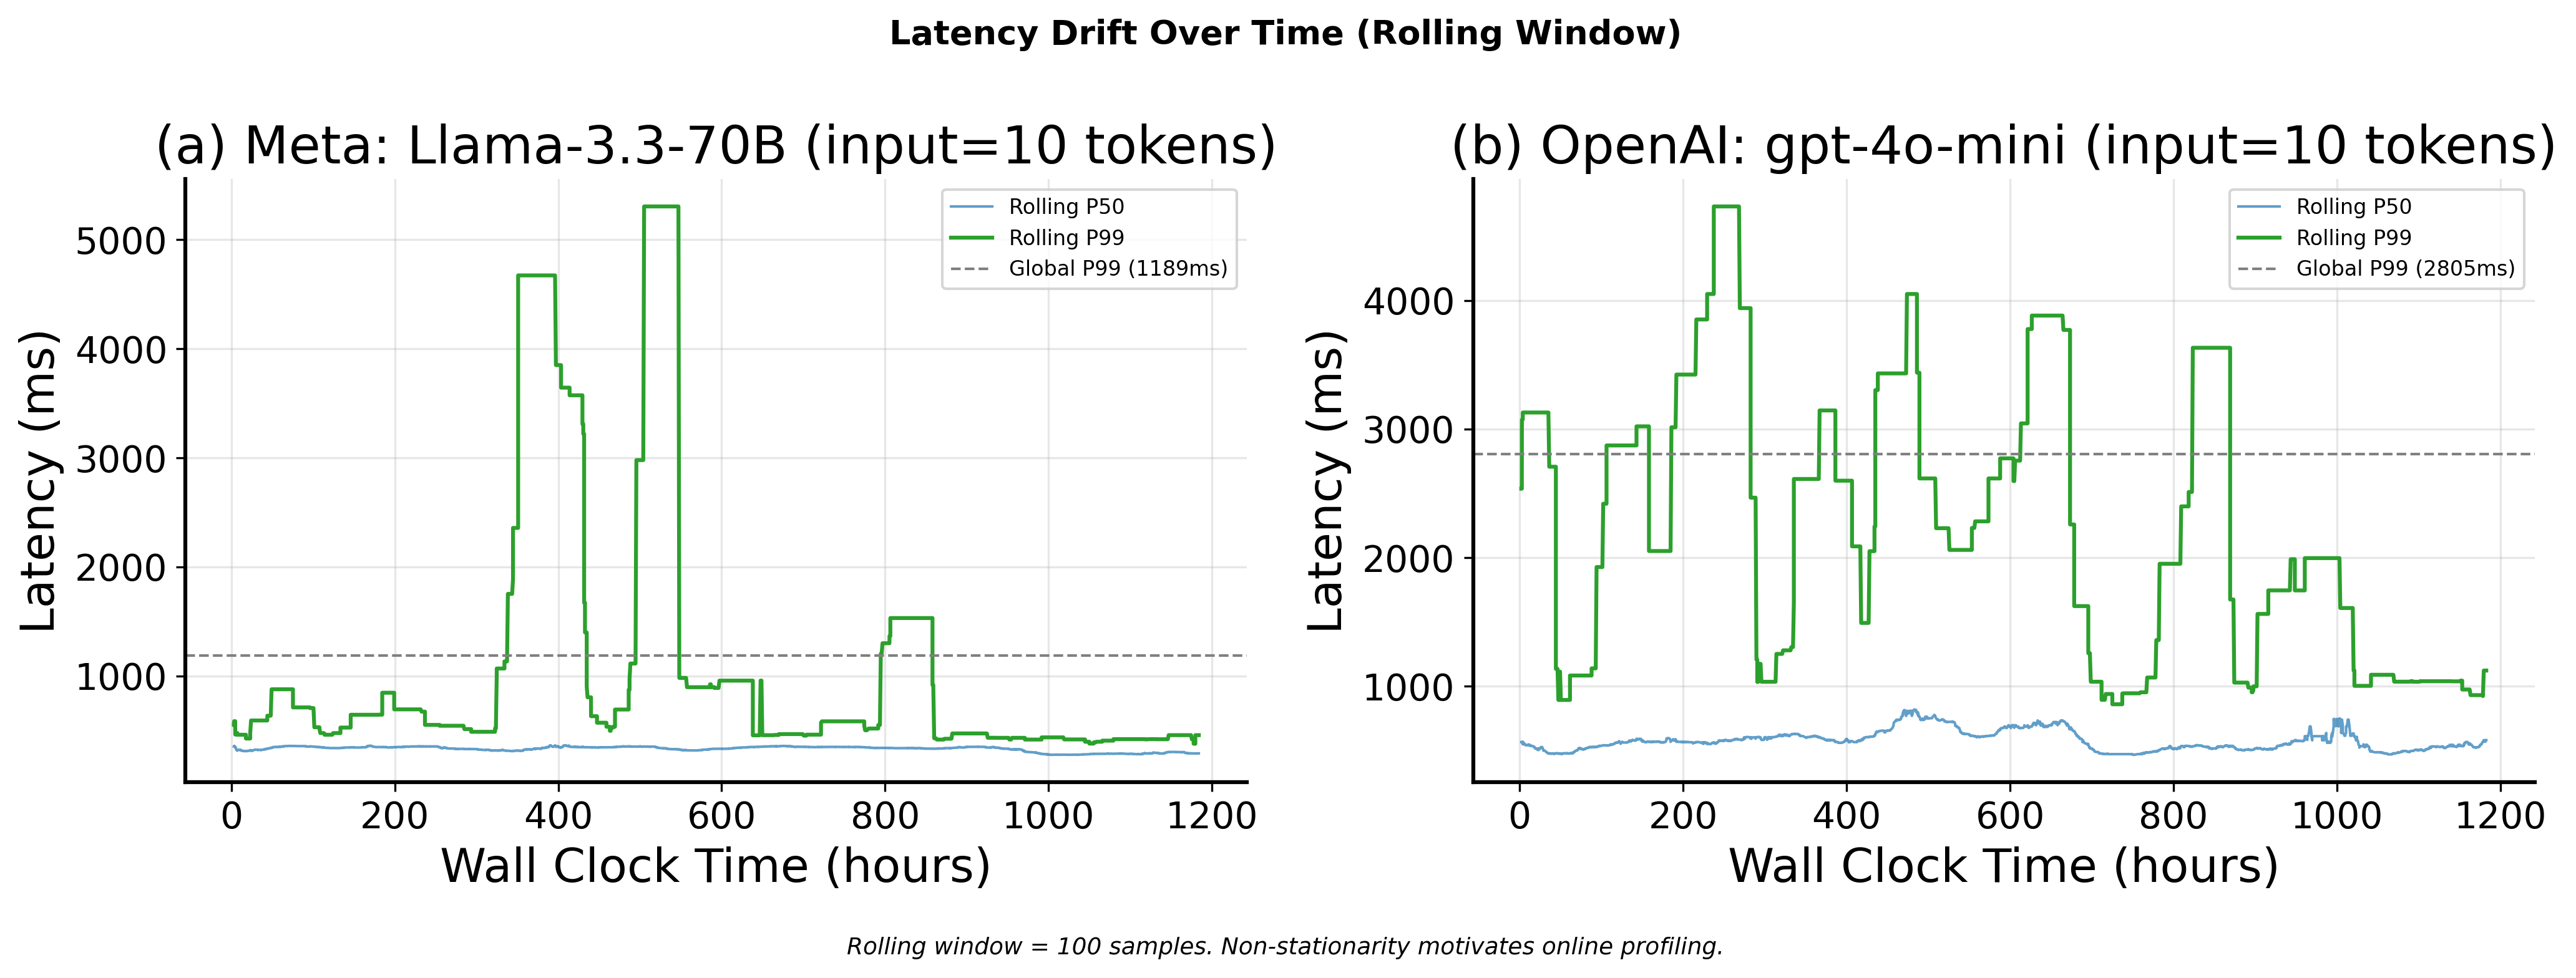
\includegraphics[width=0.95\textwidth]{images/drift_wall_clock.png}}
\caption{Provider latency over 1,200 hours. P99 latency fluctuates significantly---Meta's Llama-3.3-70B spikes from 1.2s to 5.4s, while OpenAI's GPT-4o-mini varies between 1--4.8s. The workload was collected by sending a short random prompt every 5 minutes for 50 days.}
\label{fig:latency_drift}
\end{center}
\vskip -0.2in
\end{figure*}

\paragraph{The Challenge of Opportunity Cost.}
This hybrid pricing landscape presents a classic resource allocation challenge: how to route a stream of heterogeneous requests to minimize total cost while satisfying service-level objectives (SLOs) \cite{dean_barroso_tail}. A naive greedy strategy---sending every request to a subscription until it is full---is often suboptimal. It fails to account for the \textit{opportunity cost} of consuming a scarce subscription slot with a low-value (short) request, forcing a subsequent high-value (long) request to the expensive pay-per-token API.
Consider a concrete example: a Chutes.ai subscription provides 5,000 requests per day for Llama-3.3-70B. If a user sends a trivial ``Hello'' query that would cost \$0.001 via Together API, that slot is no longer available for a complex coding request that would cost \$0.50 via API. The naive greedy policy wastes 500 $\times$ potential savings. Our experiments show that such opportunity cost losses are not merely theoretical---on real workloads, greedy routing captures only 49--83\% of the savings achievable by optimal routing (Table~\ref{tab:stage1_savings}). While motivated by the API provider marketplace, our formulation can also be applied to self-deployed GPU resource pools by modeling them as quota- and concurrency-based providers.
% \yiyan{kept one sentence here}

We address this challenge by formalizing the \textbf{Latency--Cost Optimization} problem for multi-provider LLM routing. Our contributions are:

\begin{enumerate}
    % \item \jason{add one on we categorize existing LLM inference providers into three categories, merge the first two into one} \yiyan{\textbf{Provider Taxonomy:} We categorize modern LLM inference providers into a unified set of resource types---unrestricted pay-as-you-go APIs and capacity-constrained subscriptions, where subscription constraints appear as either fixed-window quotas ($S_Q$) or reserved concurrency slots ($S_C$).}
    \item \textbf{Provider Taxonomy:} We categorize modern LLM inference providers into a unified set of resource types---unrestricted pay-as-you-go APIs ($S_A$) and capacity-constrained subscriptions, where subscription constraints appear as either fixed-window quotas ($S_Q$) or reserved concurrency slots ($S_C$).
    \item \textbf{Formal Problem Definition:} We model the routing problem under two distinct constraint types: fixed-window quotas (Stage 1) and concurrency limits (Stage 2), incorporating latency deadlines.
    \item \textbf{Offline Oracles:} We derive optimal offline algorithms for these settings. For Stage 1, we prove that a greedy-by-value strategy is optimal. For Stage 2, we formulate a time-indexed Integer Linear Program (ILP) to handle the NP-hard scheduling problem.
    \item \textbf{Online Algorithm:} We propose a Learning-Augmented Primal-Dual (LA-PD) algorithm. It uses a shadow price mechanism to value scarce resources and integrates a quantile regression model to conservatively estimate request costs under uncertainty.
    \item \textbf{Production Workload Traces:} We collect and analyze diverse LLM workloads including ShareGPT, an industry production trace, and 440K+ requests from a university campus deployment. We will release the campus trace to facilitate future research.
    \item \textbf{Empirical Results:} Using these traces, we demonstrate that our approach achieves near-optimal costs (within 1.18x of the offline oracle) and significantly outperforms standard greedy baselines.
\end{enumerate}

\section{Provider Taxonomy and Problem Formulation}
\label{sec:providers}

We model an inference marketplace as a set of services $S$ that expose the \emph{same} underlying LLMs under different pricing and capacity contracts.
Requests arrive online as a sequence $\{r_i\}$; request $r_i$ has input length $n_i^{\text{in}}$ and an \emph{a priori unknown} output length $n_i^{\text{out}}$.
Our routing decision chooses exactly one service for each request, trading off monetary cost against latency constraints.
\begin{table}[t]
\centering
\begin{tabular}{@{}lcl@{}}
\toprule
\textbf{Provider Type} & \textbf{Symbol} & \textbf{Examples} \\
\midrule
Pay-per-token API & $S_A$ & Together \\
Quota subscription & $S_Q$ & Chutes.ai \\
Concurrency subscription & $S_C$ & Featherless.ai \\
\bottomrule
\end{tabular}
\caption{Provider taxonomy for open-weight model inference (Llama, Mistral, DeepSeek-R1). Formal constraints are defined in Sections~\ref{sec:sa}--\ref{sec:sc}.}
\label{tab:provider_taxonomy}
\end{table}

\subsection{Pay-per-token APIs ($S_A$)}
\label{sec:sa}
A pay-per-token API charges a posted price per input and output token.
Routing request $r_i$ to $S_A$ incurs
\[
c_i \;=\; p_{\text{in}} \cdot n_i^{\text{in}} \;+\; p_{\text{out}} \cdot n_i^{\text{out}}.
\]
We use this service as the \emph{elastic overflow tier}: it is always feasible (no hard capacity constraint) but can be expensive at the margin.
In practice, multiple providers expose open-weight models under this pricing structure with different posted rates.\cite{together_pricing,fireworks_pricing,groq_pricing,deepseek_api_pricing}

\subsection{Quota subscriptions ($S_Q$)}
\label{sec:sq}
A quota subscription provides ``zero marginal cost'' inference up to a hard request budget within a fixed time window.
Formally, for each window, we require
\[
\sum_{i \in \text{window}} x_i^{Q} \;\le\; Q,
\]
where $x_i^{Q}\in\{0,1\}$ indicates whether request $i$ is routed to $S_Q$.
This model captures subscription tiers that impose request limits within fixed time windows (e.g., Chutes.ai with daily request quotas).\cite{chutes_pricing}
The key algorithmic challenge is \emph{opportunity cost}: allocating a scarce quota slot to a short/low-value request may force a later long/high-value request to the metered API.

\subsection{Concurrency subscriptions ($S_C$)}
\label{sec:sc}
A concurrency subscription exposes a reserved serving capacity that can process up to $C$ requests in parallel.
If request $i$ starts at time $s_i$ and occupies the server for processing time $p_i$, then the in-flight constraint is
\[
\sum_i \mathbb{I}\!\left(t \in [s_i,\, s_i+p_i]\right) \;\le\; C \quad \forall t.
\]
This captures dedicated inference endpoints with reserved capacity (e.g., Featherless.ai, Arli AI),\cite{featherless-plans,arli-pricing}
as well as self-hosted deployments in which the number of replicas bounds the number of concurrent requests.\cite{vllm_pagedattention}
Compared to $S_Q$, $S_C$ introduces scheduling structure because the resource is blocked for the request duration.

\subsection{Subscription amortization}
\label{sec:amortization}
In our experiments, we treat subscription fees as sunk costs (already paid) and optimize \emph{additional} spend on $S_A$ given fixed subscription capacities.
This matches common operational settings in which an organization has committed to subscriptions (or provisioned a cluster) and aims to maximize utilization while minimizing overflow to token-metered APIs.

\subsection{A unified abstraction beyond public APIs}
While our motivating examples come from the API marketplace, the same resource types arise in local GPU deployments.
\textbf{Concurrency as dedicated capacity:} $S_C$ maps directly to a GPU cluster with a fixed number of serving replicas, where $C$ is the maximum parallel requests.\cite{vllm_pagedattention}
\textbf{Quota as gutter pool:} $S_Q$ maps to the \textit{gutter pool}---spare GPU nodes maintained for high availability.\cite{sre_introduction_goog}
Since GPU nodes fail frequently due to hardware errors or network partitions,\cite{kokolis_reliability_2024} operators provision hot-standby capacity; routing inference to these idle nodes extracts value from sunk cost, subject to availability constraints that map to our quota model.
This unified view connects API routing to internal GPU cluster scheduling.

\subsection{Optimization objective}
\label{sec:objective}
Given a stream of requests $\mathcal{R} = \{r_1, \dots, r_T\}$, our goal is to minimize the total API cost:
\[
\min \sum_{i \in \mathcal{R}} x_i^A \cdot c_i
\]
subject to the quota constraint $\sum_{i \in \text{window}} x_i^Q \le Q$ and concurrency constraint $\sum_i \mathbb{I}(t \in [s_i, s_i+p_i]) \le C$ for all $t$, where $x_i^A, x_i^Q, x_i^C \in \{0, 1\}$ indicate routing decisions and exactly one must be 1 for each request.

\subsection{Key assumptions}
\label{sec:assumptions}
We make two simplifying assumptions.
First, \textbf{homogeneous quality}: all providers serve the same model, so routing decisions affect only cost, not output quality. This holds for open-weight models available across multiple providers.
Second, the \textbf{output token count} $n_i^{\text{out}}$ is unknown at routing time---the key source of uncertainty that motivates our learning-augmented approach.

% \section{Problem Formulation}
\label{sec:problem}

We consider a stream of inference requests $\mathcal{R} = \{r_1, r_2, \dots, r_T\}$ arriving over time. Each request $r_i$ is characterized by its arrival time $a_i$, input token count $n_i^{\text{in}}$, and (unknown at arrival) output token count $n_i^{\text{out}}$. Given the provider taxonomy defined in Section~\ref{sec:providers}, our goal is to route each request to minimize total cost while respecting capacity constraints.

\subsection{Objective}

The goal is to minimize the total API cost:
\[
\min \sum_{i \in \mathcal{R}} x_i^A \cdot c_i
\]
subject to the quota constraint $\sum_{i \in \text{window}} x_i^Q \le Q$ and concurrency constraint $\sum_i \mathbb{I}(t \in [s_i, s_i+p_i]) \le C$ for all $t$, where $x_i^A, x_i^Q, x_i^C \in \{0, 1\}$ are binary decision variables indicating where request $r_i$ is routed, and exactly one must be 1 for each request.

\subsection{Key Assumptions}

We make two simplifying assumptions. First, we assume \textbf{homogeneous quality}: all providers serve the same model, so routing decisions affect only cost, not output quality. This assumption holds for open-weight models (Llama, Mistral, DeepSeek) available across multiple providers. Second, the \textbf{output token count} $n_i^{\text{out}}$ is unknown at routing time. This is the key source of uncertainty that motivates our learning-augmented approach.
  % merged into new2-provider
\section{Optimal Offline Analysis}
\label{sec:offline}

To understand the theoretical limits of cost savings, we analyze the offline setting where the entire request sequence $\mathcal{R} = \{r_1, \dots, r_n\}$ is known in advance. We present two stages: Stage 1 considers routing between $S_Q$ and $S_A$ (quota-only), while Stage 2 incorporates the concurrency-limited subscription $S_C$, routing among all three provider types.

\subsection{Stage 1: Quota-Only Routing ($S_Q + S_A$)}
\label{sec:offline-stage1}

We first consider a simplified problem with only the quota subscription $S_Q$ and the pay-per-token API $S_A$. This provides an \textit{Economic Lower Bound}, as it ignores the concurrency-limited resource.

\textbf{Problem Formulation.}
Let $x_i^Q \in \{0,1\}$ indicate whether request $i$ is routed to $S_Q$. The objective is to maximize total avoided API cost:
\begin{equation}
    \max \sum_{i \in \mathcal{R}} x_i^Q \cdot c_i^{\text{API}}
\end{equation}
subject to the quota constraint for each window $k$:
\begin{equation}
    \sum_{i: \operatorname{win}(a_i)=k} x_i^Q \le Q_{\text{win}}, \quad \forall k
\end{equation}

\textbf{Optimal Solution.}
Since each request consumes exactly one unit of quota, this problem decomposes into independent selection problems (one per window) where all item weights are 1. The optimal strategy is to route the $Q_{\text{win}}$ requests with the highest API costs to $S_Q$ in each window.

\begin{theorem}
For the Quota-Only problem, the Greedy-by-Value strategy is optimal and can be computed in $\mathcal{O}(n \log n)$ time.
\end{theorem}

\subsection{Stage 2: Full Routing ($S_Q + S_C + S_A$)}
\label{sec:offline-stage2}

When we add the concurrency-limited subscription $S_C$, requests can be routed to any of the three providers. The problem becomes NP-hard, coupling quota allocation with parallel machine scheduling.

\textbf{ILP Formulation.}
We formulate this as a time-indexed Integer Linear Program (ILP). We discretize time into slots $t \in \{0, \dots, T\}$ of width $\Delta$. Let $\alpha_i$ and $\beta_i$ denote the earliest and latest feasible start slots for request $i$, and let $\hat{p}_i = \lceil p_i / \Delta \rceil$ be its processing time in slots. Define $z_{i,t} \in \{0,1\}$ to indicate if request $i$ starts on $S_C$ at slot $t$.

The objective is to minimize total API cost:
\begin{equation}
    \min \sum_{i \in \mathcal{R}} x_i^A \cdot c_i^{\text{API}}
\end{equation}

Subject to:
\begin{align}
    & x_i^Q + x_i^C + x_i^A = 1, \quad \forall i \label{eq:assign} \\
    & \sum_{i: \operatorname{win}(a_i)=k} x_i^Q \le Q_{\text{win}}, \quad \forall k \label{eq:quota} \\
    & \sum_{t=\alpha_i}^{\beta_i} z_{i,t} = x_i^C, \quad \forall i \label{eq:consistency} \\
    & \sum_{i \in \mathcal{R}} \sum_{\tau=\max(\alpha_i, t-\hat{p}_i+1)}^{\min(\beta_i, t)} z_{i,\tau} \le C, \quad \forall t \label{eq:concurrency}
\end{align}

Constraint~(\ref{eq:assign}) ensures each request is routed to exactly one provider. Constraint~(\ref{eq:quota}) enforces the quota limit per window. Constraint~(\ref{eq:consistency}) links routing decisions to scheduling variables. Constraint~(\ref{eq:concurrency}) enforces the instantaneous concurrency limit. Full details including deadline handling are in Appendix~\ref{app:stage2_ilp}.

This ILP provides the \textit{Physical Lower Bound}. The gap between Stage 1 and Stage 2 costs quantifies the \textit{Cost of Concurrency}---efficiency lost due to physical resource contention when $S_C$ cannot absorb all high-value requests.

\section{Online Routing Algorithms}
\label{sec:online}

In the online setting, we must make irrevocable routing decisions without knowledge of future arrivals or exact output lengths. We propose a unified framework that combines primal-dual algorithm design with learning-augmented predictions.

\subsection{Primal-Dual Framework}

We treat the subscription capacity as a scarce resource and assign it a dynamic \textit{shadow price}. This price represents the opportunity cost of using a subscription slot.

\textbf{Quota Shadow Price ($\psi$).}
For the daily quota constraint ($S_Q$), let $z = k/Q$ be the fraction of quota consumed. We define an exponential threshold function $\psi(z)$:
\begin{equation}
    \psi(z) = L \cdot \left( \frac{U}{L} \right)^z
\end{equation}
where $L$ and $U$ are estimated lower and upper bounds on the request value (avoided API cost). A request is routed to $S_Q$ only if its value exceeds this threshold.

\begin{theorem}[Competitive Ratio]
The primal-dual algorithm with threshold $\psi(z)$ achieves a competitive ratio of $O(\ln(U/L))$ for the online knapsack problem with known values.
\end{theorem}

\textbf{Remark.} The theorem assumes exact request values are known at arrival. In practice, we use predicted values $\hat{v}_t$, so the guarantee applies to the \emph{estimated} value sequence. Actual performance depends on prediction quality; we validate this empirically in Section~\ref{sec:experiments}.

\textbf{Concurrency Shadow Price ($\lambda$).}
For the concurrency constraint ($S_C$), we define a congestion price $\lambda_t$ based on the current utilization of the concurrency slots. When the system is saturated (queue full or utilization high), $\lambda_t$ increases, admitting only requests with high \textit{value density} (value per unit time).
\begin{equation}
    \lambda_t = \begin{cases}
    0 & \text{if capacity available} \\
    \min_{r \in \text{Queue}} \frac{v(r)}{w(r) \cdot p(r)} & \text{if saturated}
    \end{cases}
\end{equation}

\subsection{Learning-Augmented Decision Making}

A key challenge is that the ``value'' of a request (its output token count $n_i^{\text{out}}$) is unknown at arrival time. Standard estimators (e.g., historical averages) can be risky: over-estimating value leads to wasting scarce quota on cheap requests.

We employ a \textbf{Learning-Augmented} approach with two components. First, we use \textbf{quantile regression} to train a lightweight model that predicts the distribution of output tokens. Specifically, we predict the 10th percentile (P10) $\hat{L}^{(10)}_t$ and the median (P50) $\hat{L}^{(50)}_t$. Second, we use \textbf{conservative value estimation} via the Lower Confidence Bound (LCB). We estimate the request value using the P10 prediction:
\begin{equation}
    \hat{v}_t^{\text{LCB}} = p_{\text{in}} \cdot n_t^{\text{in}} + p_{\text{out}} \cdot \hat{L}^{(10)}_t
\end{equation}
This conservative estimate ensures that the request is worth at least this much before spending quota on it.

\textbf{Duration Estimation.}
For concurrency-aware routing, we also need to estimate the processing time $\hat{p}_t$. We decompose this as $\hat{p}_t \approx \widehat{\text{TTFT}} + \hat{n}_t^{\text{out}} / \widehat{\text{TPS}}$, where TTFT is time-to-first-token and TPS is decode throughput. To avoid underestimating slot occupancy, we use upper confidence bounds (90th percentile for TTFT and output length, 10th percentile for TPS). Details are in Appendix~\ref{app:duration}.

\subsection{Unified Risk-Aware Routing Algorithm}

We combine the shadow prices and the conservative value estimate into a unified decision rule. For each incoming request $r_t$, we calculate the \textbf{net gain} of each routing option separately:
\begin{align}
    G_Q &= \hat{v}_t^{\text{LCB}} - \psi(z_t) \label{eq:gain_q} \\
    G_C &= \hat{v}_t^{\text{LCB}} - \lambda_t \cdot w_t \cdot \hat{p}_t \label{eq:gain_c} \\
    G_A &= 0 \quad \text{(baseline)} \label{eq:gain_a}
\end{align}
where $w_t$ is the concurrency weight (typically 1, but larger for models requiring more GPU memory). The router selects $\arg\max\{G_Q, G_C, G_A\}$, subject to capacity constraints.

\begin{algorithm}[tb]
   \caption{Unified Risk-Aware Routing (LA-PD)}
   \label{alg:lapd}
\begin{algorithmic}
   \STATE {\bfseries Input:} Request $r_t$, quota usage $k_t$, concurrency state
   \STATE {\bfseries Parameters:} Quota $Q$, concurrency $C$, value bounds $[L, U]$
   \STATE 1. Predict $\hat{n}_t^{\text{out}} \gets \mathcal{M}(r_t)$; estimate $\hat{v}_t^{\text{LCB}}$, $\hat{p}_t$
   \STATE 2. Compute shadow prices: $\psi(z_t) \gets L \cdot (U/L)^{k_t/Q}$, $\lambda_t$
   \STATE 3. Compute net gains: $G_Q$, $G_C$, $G_A$ via Eq.~\eqref{eq:gain_q}--\eqref{eq:gain_a}
   \STATE 4. Set $G_Q \gets -\infty$ if $k_t \geq Q$; $G_C \gets -\infty$ if incompatible
   \IF{$G_Q \geq G_C$ \AND $G_Q > 0$}
       \STATE Route to $S_Q$; update $k_{t+1} \gets k_t + 1$
   \ELSIF{$G_C > 0$}
       \STATE Route to $S_C$; update concurrency state
   \ELSE
       \STATE Route to API ($S_A$)
   \ENDIF
\end{algorithmic}
\end{algorithm}

\section{Latency-Aware Provider Selection}
\label{sec:latency}

While the preceding sections optimize for cost, practical deployments must also satisfy latency Service Level Objectives (SLOs). When multiple providers serve the same model through platforms like OpenRouter, their latency profiles differ substantially---motivating a separate optimization dimension orthogonal to cost.

\subsection{Problem Setting}

Given a set of providers $\mathcal{P} = \{1, \ldots, n\}$ serving the same model, each provider $j$ has:
\begin{itemize}
    \item Cost per request $c_j$ (from token pricing)
    \item Latency distribution $F_j(\cdot)$ estimated from online probing
\end{itemize}

The goal is to find routing probabilities $\pi = (\pi_1, \ldots, \pi_n)$ that minimize expected cost while satisfying a tail latency constraint (e.g., P99 $\leq L$).

\subsection{Online Latency Profiling}

Provider latencies exhibit high variance and temporal drift due to changing queue depths. We maintain per-provider latency profiles using a \textbf{mixed-window estimator}:
\begin{equation}
    \hat{F}_j(L) = \beta \cdot F_j^{\text{short}}(L) + (1 - \beta) \cdot F_j^{\text{long}}(L)
\end{equation}
where $F_j^{\text{short}}$ is the empirical CDF from a 15-minute window (responsive to drift), $F_j^{\text{long}}$ is from a 3-hour window (stable prior), and $\beta$ is an adaptive shrinkage weight. Profiles are updated via lightweight probing every 45 seconds per provider.

\subsection{LP-Based Provider Mixing}

Given latency profiles, we solve for the optimal routing mix via linear programming:
\begin{align}
\min_{\pi} \quad & \sum_{j \in \mathcal{P}} \pi_j c_j \label{eq:lp_obj} \\
\text{s.t.} \quad & \sum_{j \in \mathcal{P}} \pi_j F_j(L) \geq 1 - \alpha \label{eq:lp_slo} \\
& \sum_{j \in \mathcal{P}} \pi_j = 1, \quad \pi_j \geq 0 \nonumber
\end{align}
where $L$ is the SLO threshold and $\alpha$ is the target violation rate (e.g., $\alpha = 0.01$ for P99). Constraint~\eqref{eq:lp_slo} ensures the mixture CDF at $L$ exceeds $1 - \alpha$.

\begin{proposition}[Sparsity of Optimal Mix]
\label{prop:lp_sparsity}
The optimal solution to the LP~\eqref{eq:lp_obj}--\eqref{eq:lp_slo} has at most 2 non-zero components.
\end{proposition}

\textbf{Proof.} See Appendix~\ref{app:lp_sparsity_proof}.

This sparsity is practically valuable: routing decisions involve choosing between at most two providers, simplifying implementation and reducing variance.

\subsection{Smart Hedging for Tail Guarantees}

LP mixing optimizes the \textit{expected} latency distribution but cannot guarantee individual request SLOs. We augment it with a \textbf{smart hedging} mechanism that sends a backup request to a faster provider when the primary is at risk of violating the SLO.

\textbf{Survival-Based Decision Rule.}
Let $t$ be the elapsed time since a request was sent. Define the survival function $S(x) = 1 - F(x) = P(T > x)$. We trigger a hedge when the conditional probability of violating the SLO by waiting exceeds the probability of violating by hedging:
\begin{equation}
    \frac{S_{\text{primary}}(L)}{S_{\text{primary}}(t)} > S_{\text{backup}}(L - t - \delta)
    \label{eq:hedge_survival}
\end{equation}
where $\delta$ is the dispatch overhead. This triggers hedging only when it reduces the expected violation probability.

\textbf{Implementation.}
We compute a hedge threshold $h^*$ as the smallest $t$ satisfying~\eqref{eq:hedge_survival} under the current online profiles. If the primary request has not completed by $h^*$, we dispatch a backup request and return the first response.

\textbf{Cost Overhead.}
Without cancellation, both requests may be billed, so the expected overhead scales with the hedge rate and the backup-to-primary cost ratio. Many providers support request cancellation by closing the HTTP connection, which can stop further token generation and reduce wasted cost; Appendix~\ref{app:cancel_aware} provides a cancel-aware cost model and empirical results.

\subsection{Integration with Cost Routing}

Latency-aware selection operates orthogonally to cost routing (Section~\ref{sec:online}). After the cost router decides to use the API provider $S_A$, the latency module selects \textit{which} API provider within $S_A$ to use:
\begin{enumerate}
    \item Cost router decides: $S_Q$, $S_C$, or $S_A$
    \item If $S_A$: Latency router selects provider $j \sim \pi^*$ via LP mixing
    \item Monitor elapsed time; hedge if survival condition~\eqref{eq:hedge_survival} triggers
\end{enumerate}

This modular design allows independent optimization of cost and latency while maintaining a simple, interpretable system.

\section{Experiments}
\label{sec:experiments}

We evaluate our proposed algorithms on real-world traces to answer three key questions: (1) What is the economic potential of optimal routing? (2) Can our online algorithms approach offline optimal under uncertainty? (3) Does latency-aware routing with hedging reduce SLO violations in production?

\subsection{Setup}

\paragraph{Datasets.} We use three real-world datasets plus one synthetic trace (Table~\ref{tab:datasets}). \textbf{ShareGPT} (201K requests) represents standard chatbot workloads. \textbf{FreeInference} (371K requests) represents diverse API gateway traffic with high variance. \textbf{Enterprise} (55K requests) is an anonymized production coding assistant with long contexts and the highest cost variance (CV $> 2$). \textbf{BurstGPT} (1.4M requests) combines BurstGPT arrival timestamps with ShareGPT prompts for online evaluation.

\begin{table}[h]
\caption{Dataset Statistics}
\label{tab:datasets}
\vskip 0.1in
\begin{center}
\begin{small}
\begin{tabular}{@{}lrrrrr@{}}
\toprule
Dataset & Reqs & Days & Models & In & Out \\
\midrule
ShareGPT & 201K & 7 & 1 & 156 & 423 \\
FreeInference & 371K & 90 & 12 & 892 & 1247 \\
Enterprise & 55K & 84 & 8 & 2341 & 3892 \\
BurstGPT & 1.4M & 61 & 1 & 234 & 512 \\
\bottomrule
\end{tabular}
\end{small}
\end{center}
\vskip -0.1in
\end{table}

\paragraph{Baselines and Pricing.} We compare against \textbf{All-API} (cost upper bound), \textbf{Greedy} (FCFS to subscription), and \textbf{Offline Optimal} (Stage 1/2 oracles). Pricing follows DeepSeek-R1: \$0.55/1M input, \$2.19/1M output tokens.

\subsection{Cost Efficiency}

\paragraph{Quota-Based Routing (Stage 1).}
With quota constraints alone, Greedy routing saves 17--81\% across datasets, while Optimal achieves 35--98\%---Greedy captures only 49--83\% of optimal savings. The gap is largest on high-variance workloads (Enterprise: CR 4.36$\times$), confirming that opportunity cost matters. Figure~\ref{fig:sensitivity} shows this gap widens with quota size: as quota increases, Optimal becomes more selective while Greedy continues wasting slots on low-value requests.

\begin{figure*}[t]
\vskip 0.1in
\begin{center}
\centerline{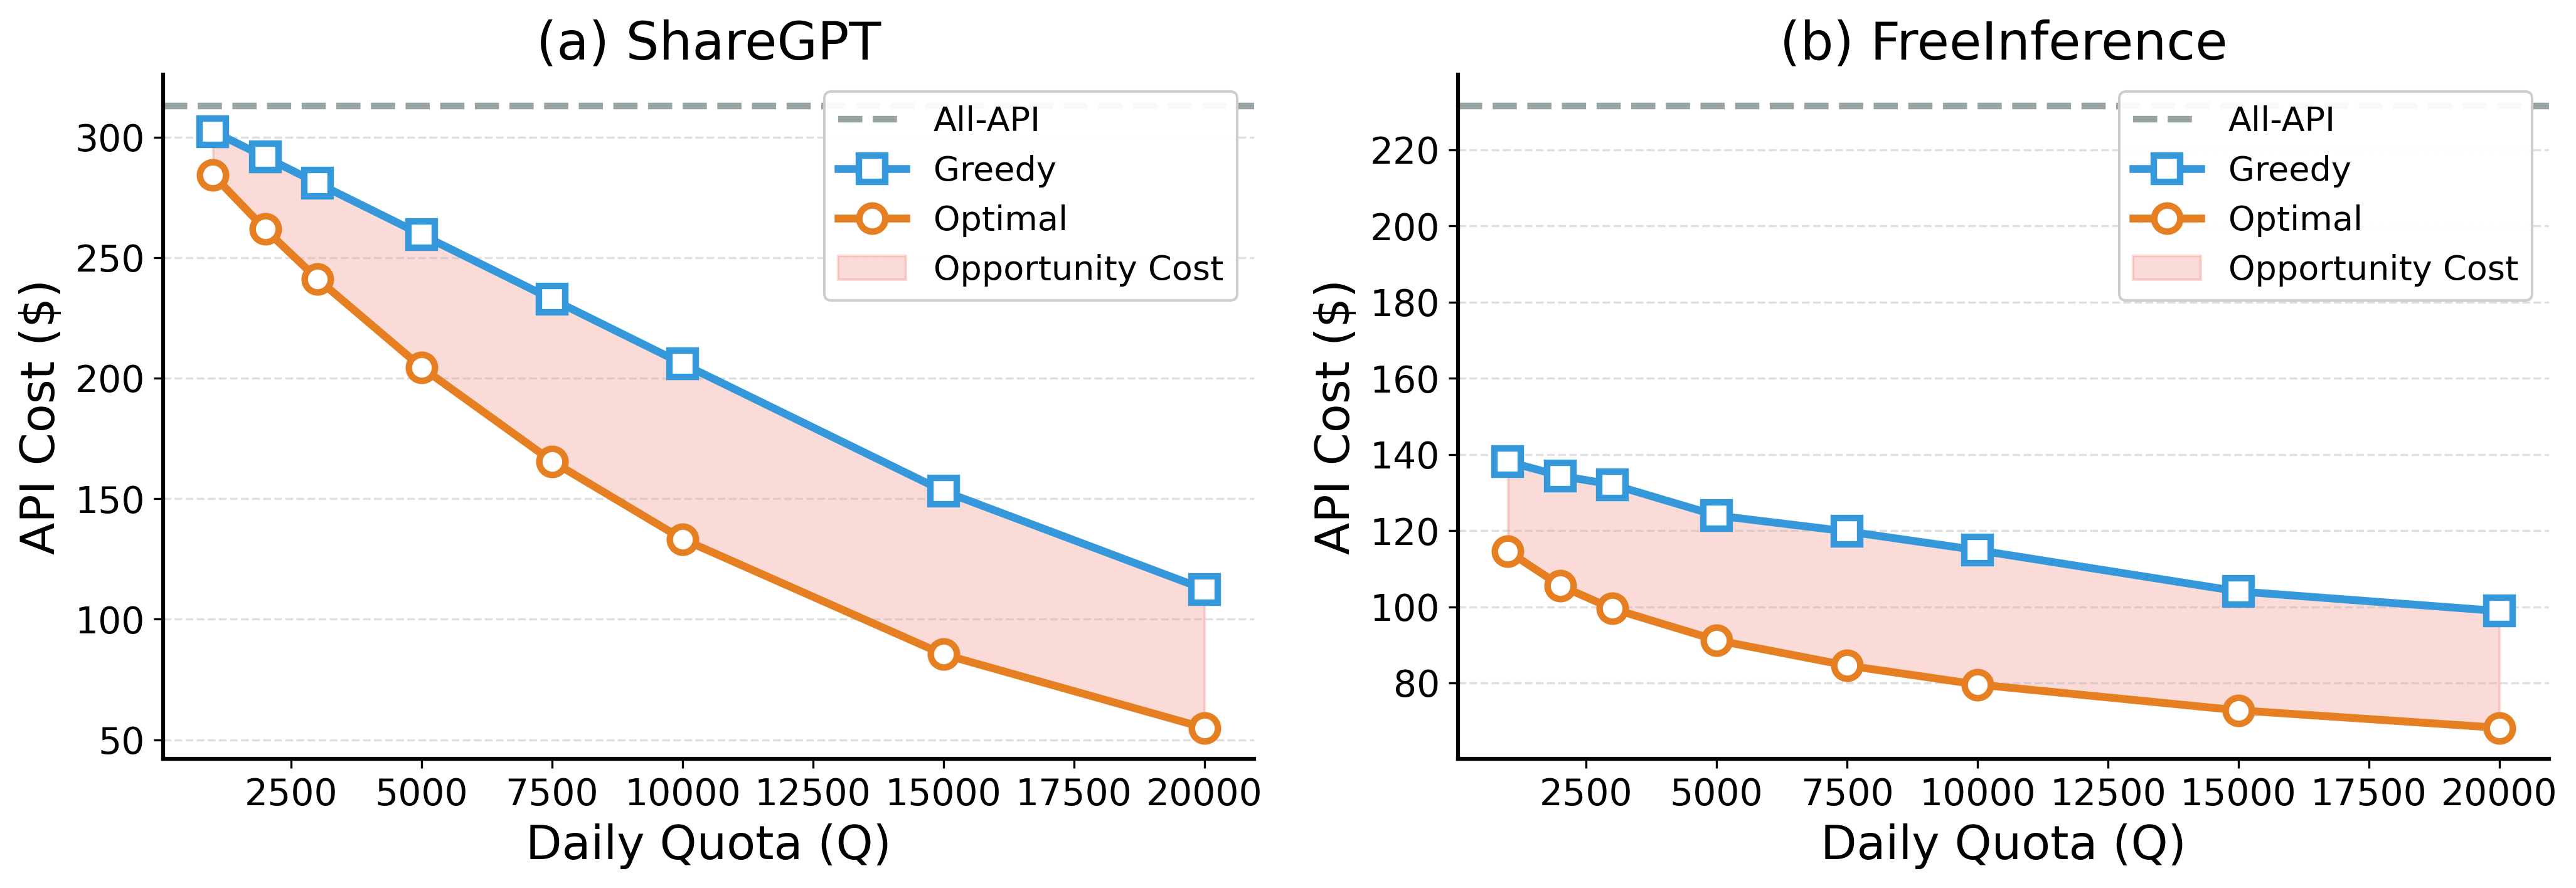
\includegraphics[width=0.95\textwidth]{images/fig2_sensitivity_combined.png}}
\caption{API cost vs quota size. The gap between Greedy and Optimal widens as quota increases, especially for multi-model workloads. The shaded area represents the opportunity cost that Greedy fails to capture.}
\label{fig:sensitivity}
\end{center}
\vskip -0.2in
\end{figure*}

\paragraph{Concurrency Constraints (Stage 2).}
For small models (e.g., Llama-3-8B), concurrency limits rarely bind before quota exhaustion. However, for larger models (70B+) with low effective concurrency ($C_{\text{eff}}=2$), physical constraints become binding (Figure~\ref{fig:concurrency_impact}). The ILP-based Stage 2 routing becomes essential.

\begin{figure}[ht]
\vskip 0.1in
\begin{center}
\centerline{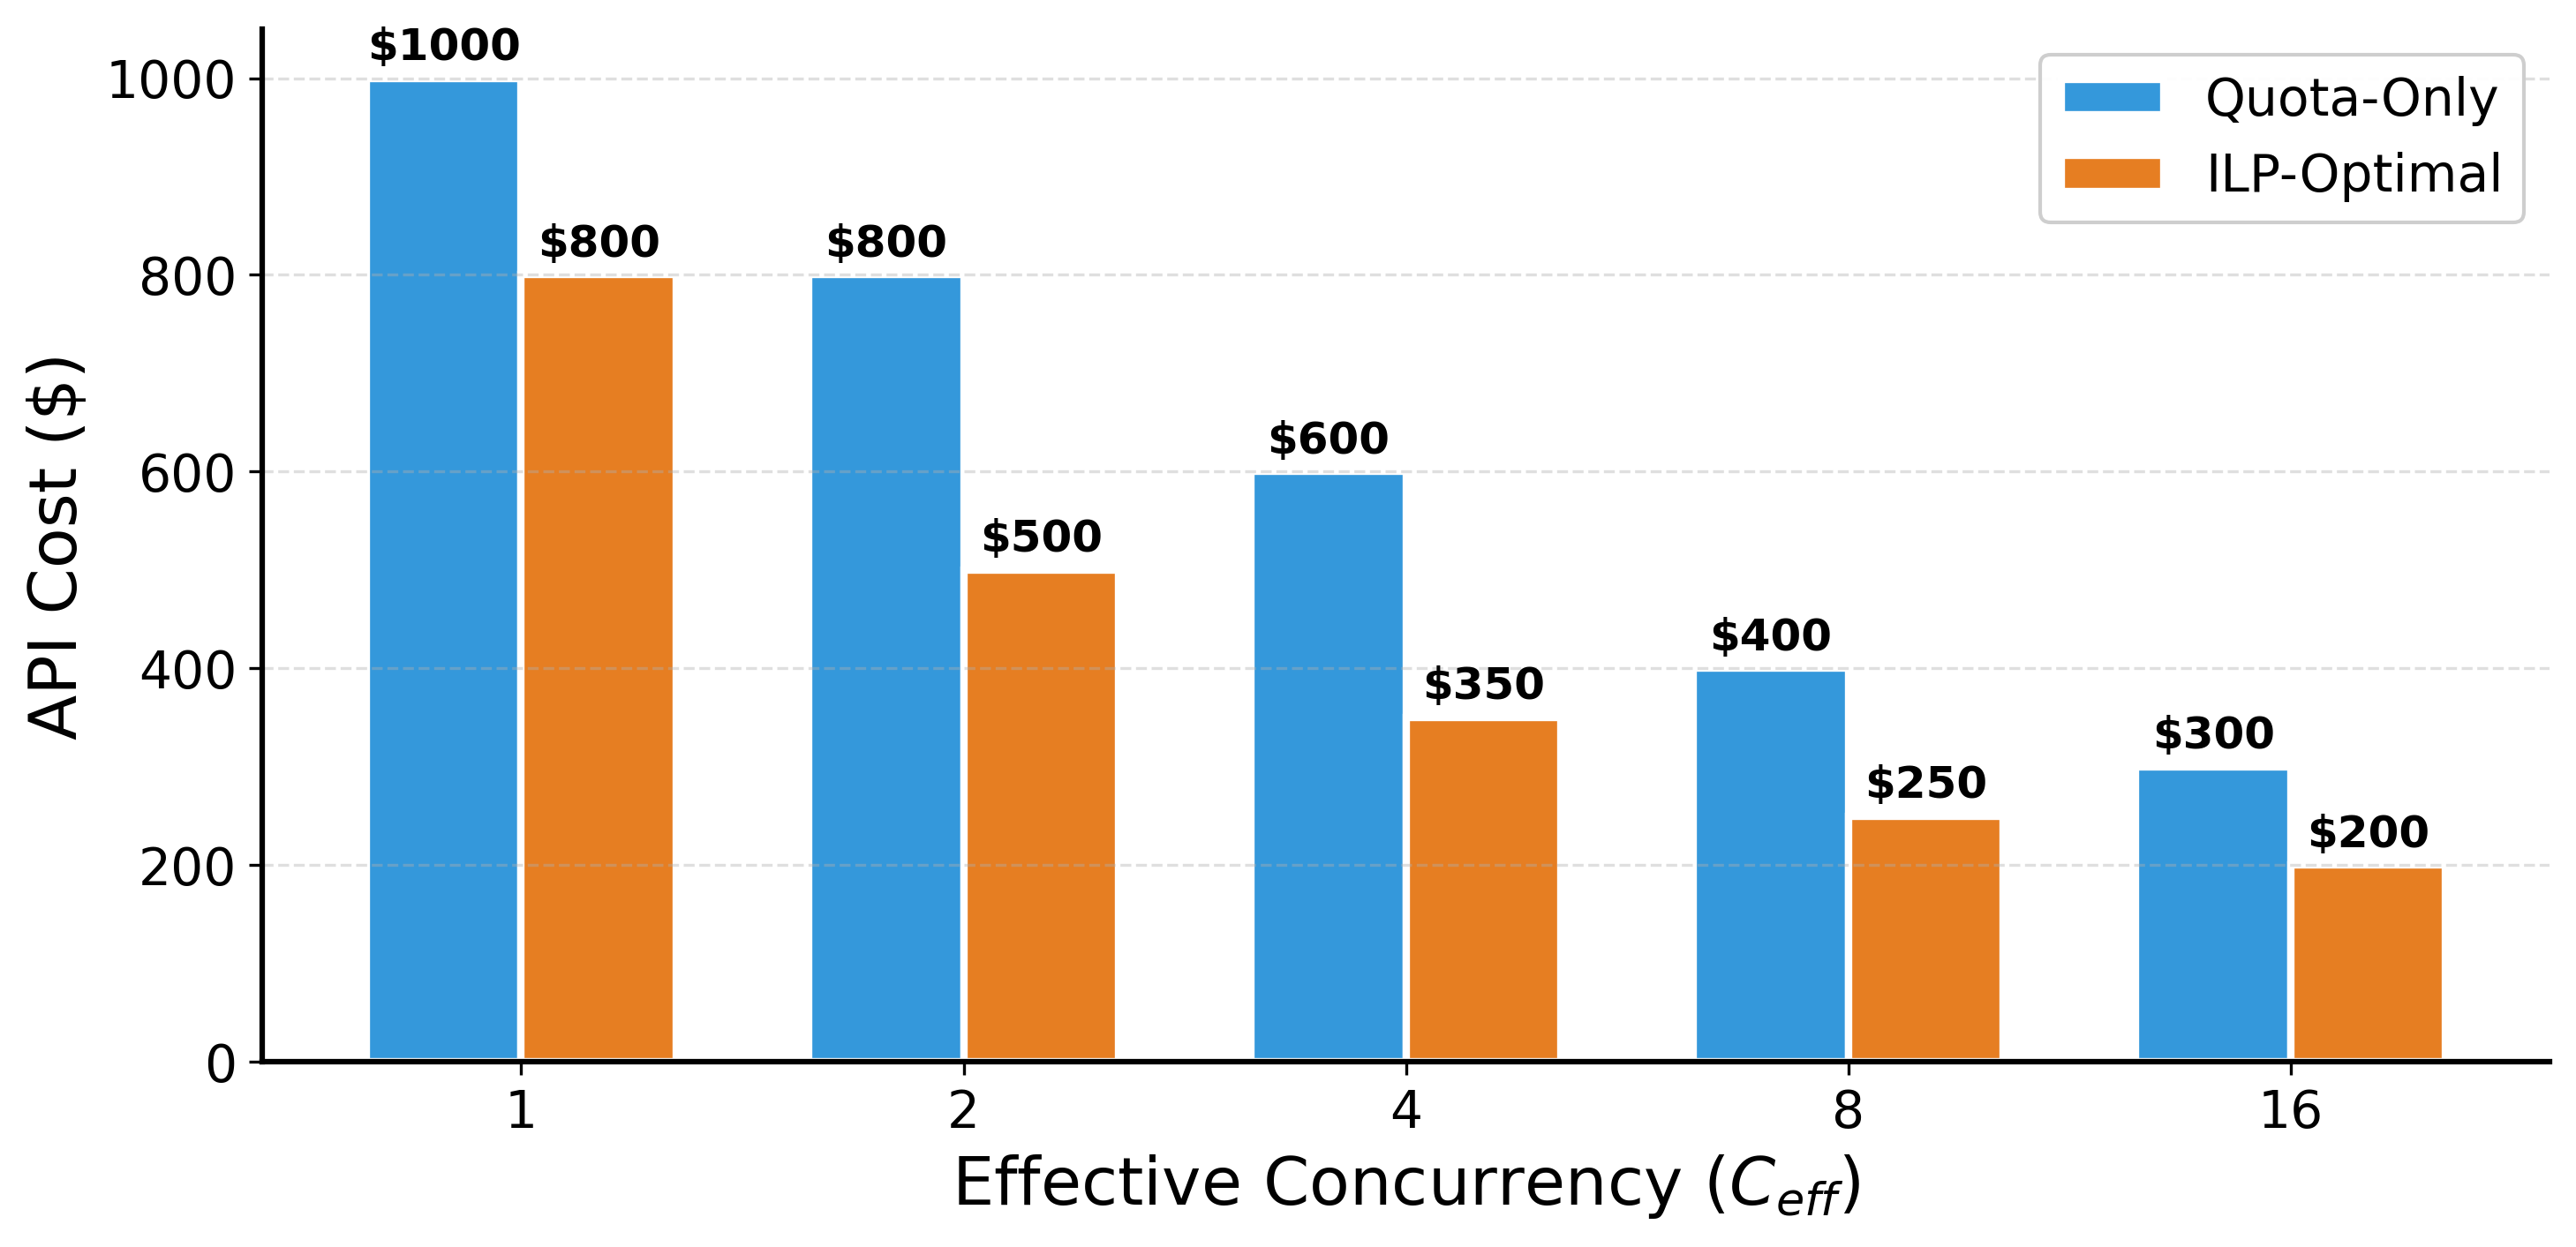
\includegraphics[width=\columnwidth]{images/single_model_comparison_rednote.png}}
\caption{Impact of model size on cost. As effective concurrency decreases, the gap between Quota-Only and ILP-Optimal widens.}
\label{fig:concurrency_impact}
\end{center}
\vskip -0.2in
\end{figure}

\paragraph{Online Joint Optimization.}
On Enterprise (54K requests, $C=8$), our PrimalDual algorithm achieves 99\% savings with CR 0.57$\times$---\textit{surpassing} the ILP-Optimal (1.0$\times$). This counterintuitive result arises because ILP discretizes time into 1-second slots, causing capacity fragmentation. PrimalDual's continuous-time event-driven admission captures opportunities that batch optimization misses. For comparison, $S_Q$-Only saves only 2\% (quota insufficient when costs vary), $S_C$-Only saves 68\% (powerful but scheduling-limited), and Greedy achieves 98\%.

\subsection{Robustness Under Uncertainty}

\paragraph{Online Performance.}
On BurstGPT (1.4M requests), our PD-EMA algorithm achieves CR 1.18$\times$, approaching the theoretical limit and outperforming Greedy (1.30$\times$). The learning-augmented variant LA-PD achieves 1.19$\times$---slightly worse than the simpler EMA approach.

\paragraph{Predictor Analysis.}
A 2$\times$2 ablation crossing predictors (EMA vs Histogram) with decision rules (Primal-Dual vs LA-PD) reveals that EMA + Primal-Dual achieves the best CR (1.18), while all other combinations achieve 1.19. Calibration analysis (Figure~\ref{fig:calibration}) explains this paradox: EMA's q50 coverage is 72\% (over-estimation), while Histogram achieves 56\% (near-ideal). Yet EMA performs better because its over-estimation naturally implements a conservative policy, and it adapts quickly to distribution shifts. For routing, \textbf{responsiveness trumps calibration}.

\begin{figure}[ht]
\vskip 0.1in
\begin{center}
\centerline{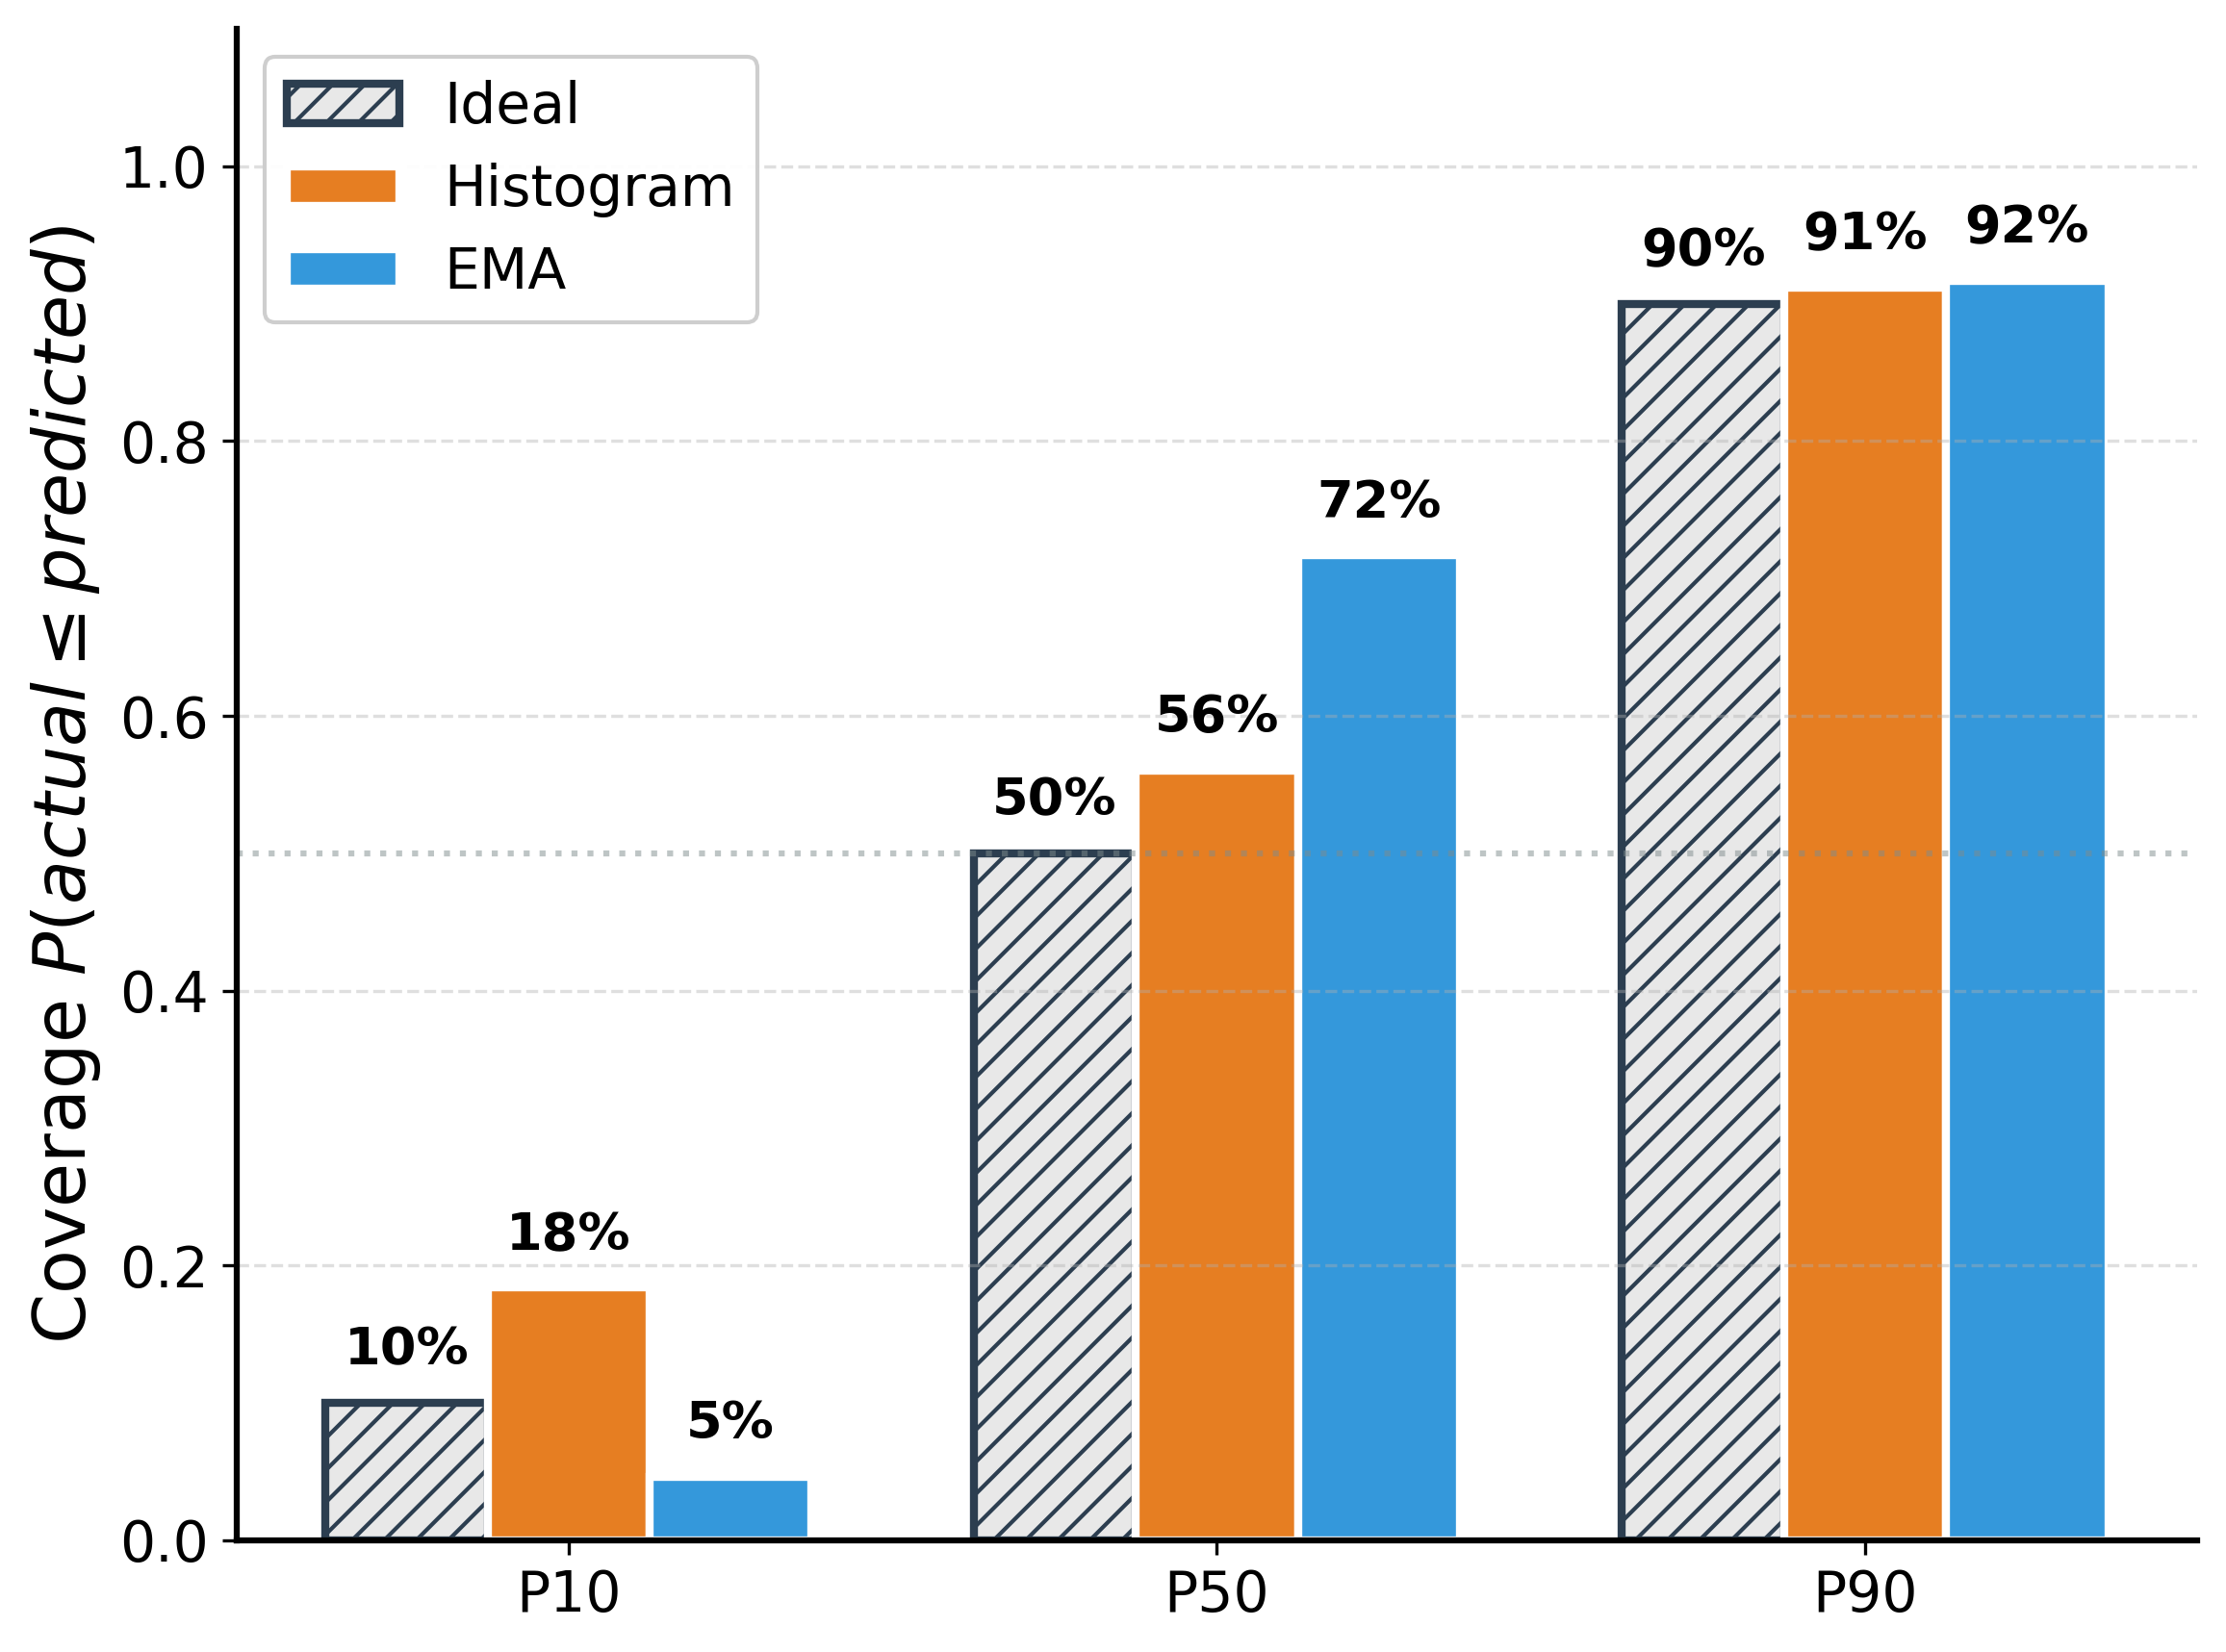
\includegraphics[width=0.85\columnwidth]{images/online_calibration.png}}
\caption{Predictor calibration. Histogram is better calibrated (closer to diagonal), but EMA achieves better routing due to faster adaptation to distribution shifts.}
\label{fig:calibration}
\end{center}
\vskip -0.2in
\end{figure}

\subsection{Latency-Aware Routing}

We evaluate latency-aware routing on OpenRouter, serving Llama-3.3-70B-Instruct across 12+ providers.

\paragraph{Provider Heterogeneity.}
Probing 12 providers over 24 hours ($n \approx 11$K samples each) reveals P99 latencies ranging from 796ms (Groq) to 16,149ms (Hyperbolic)---a 20$\times$ variation. Even providers with similar medians differ substantially in tail behavior (CV ranges 0.60--4.75), motivating online profiling over static configuration.

\paragraph{LP-Based Mixing.}
We solve for routing fractions $\pi_j$ minimizing cost subject to $\sum_j \pi_j F_j(L) \geq 0.99$ (P99 SLO at threshold $L$). At tight SLOs (2s), optimal mix favors Groq (fast, expensive); as SLO relaxes to 5s, traffic shifts to cheaper providers, reducing cost by 3$\times$ (see Figure~\ref{fig:latency_pareto} in Appendix).

\paragraph{Smart Hedging.}
To guarantee tail latency without over-provisioning, we trigger backup requests when elapsed time exceeds the primary provider's P90 threshold. Simulation shows residual-based hedging eliminates SLO violations with only 3\% cost overhead, while always-hedging costs 3.3$\times$ more.

\paragraph{Production Evaluation.}
We replay a 24-hour trace (BurstGPT timestamps + ShareGPT prompts) against the live OpenRouter API, sending each request to all policies simultaneously for fair comparison. Table~\ref{tab:openrouter_comparison} shows results.

\begin{table}[ht]
\caption{24-Hour Evaluation vs OpenRouter (SLO = 2s)}
\label{tab:openrouter_comparison}
\vskip 0.1in
\begin{center}
\begin{small}
\begin{tabular}{@{}lrrrr@{}}
\toprule
Policy & P50 & P99 & Viol. & Cost \\
\midrule
OpenRouter Auto & 820ms & 7828ms & 23.8\% & \$1.81 \\
LP-Mix & 418ms & 3659ms & 5.3\% & \$0.98 \\
Smart Hedge & 419ms & 1431ms & 0.8\% & \$1.15 \\
\bottomrule
\end{tabular}
\end{small}
\end{center}
\vskip -0.1in
\end{table}

Smart Hedge reduces SLO violations by \textbf{31$\times$} (0.8\% vs 23.8\%) and P99 latency by \textbf{5.5$\times$} (1.4s vs 7.8s) compared to OpenRouter's default routing, while saving \textbf{37\%} cost (\$1.15 vs \$1.81). Hedging triggered on 15.6\% of requests, demonstrating selective activation. LP-Mix alone achieves 46\% cost savings but higher tail latency; smart hedging trades modest cost for dramatically better latency guarantees.

\section{Related Work}
\label{sec:related}

\paragraph{LLM Routing and Cascading.}
A growing body of work routes queries across \textit{different} LLMs to optimize quality--cost tradeoffs.
FrugalGPT~\cite{chen2023frugalgptuselargelanguage} proposes LLM cascades that sequentially query cheaper models first and escalate only when confidence is low, matching GPT-4 quality at up to 98\% cost reduction.
RouteLLM~\cite{ong2025routellmlearningroutellms} trains router models from human preference data to dynamically select between a stronger and weaker LLM.
Dekoninck et al.~\cite{dekoninck2025unifiedapproachroutingcascading} unify routing and cascading into a single framework with provably optimal strategies.
AutoMix~\cite{aggarwal2025automixautomaticallymixinglanguage} uses self-verification and a POMDP-based router for model selection.
All of these works exploit \textit{quality heterogeneity} across models with different capabilities.
In contrast, our work exploits \textit{pricing heterogeneity} across providers serving the \textit{identical} model---routing decisions affect cost and latency, not output quality.
To the best of our knowledge, no prior work addresses same-model cross-provider routing under heterogeneous pricing structures.

\paragraph{Multi-Cloud and Spot Instance Serving.}
SkyPilot~\cite{DBLP:conf/nsdi/YangWLCBKZLMSS23} brokers ML workloads across clouds by optimizing instance selection for cost and availability.
SkyServe~\cite{DBLP:conf/eurosys/MaoXWCGBYSS25} extends this to AI model serving, using a SpotHedge policy that places replicas across regions and clouds with spot instances to reduce cost by 43\% while improving tail latency.
SpotServe~\cite{miao2023spotserveservinggenerativelarge} serves LLMs on preemptible instances with dynamic reparallelization and stateful recovery.
These systems operate at the \textit{infrastructure level}---managing VMs, GPU instances, and model replicas.
Our work operates at the \textit{API level}: we take provider endpoints as given and make per-request routing decisions under heterogeneous pricing contracts (pay-per-token, quota, concurrency), a complementary abstraction that does not require infrastructure control.

\paragraph{LLM Serving Systems.}
Recent systems optimize throughput and latency within individual serving instances: vLLM~\cite{vllm_pagedattention} introduces PagedAttention for efficient KV-cache management, SGLang~\cite{sglang_radixattention} uses RadixAttention for prefix caching, Orca~\cite{orca_osdi22} pioneered continuous batching, and DistServe~\cite{distserve_osdi24} disaggregates prefill and decoding for goodput optimization.
Our work is complementary, optimizing the \textit{routing layer} across multiple provider endpoints rather than the serving engine within a single endpoint.

\paragraph{Online Algorithms.}
Our work builds on the \textit{ski-rental problem}~\cite{karlin_ski_rental_algorithmica94}---the canonical rent-vs-buy decision under uncertainty---and the \textit{online knapsack problem}~\cite{han_online_knapsack_tcs15} for packing items into limited capacity.
The primal-dual framework~\cite{buchbinder_naor_pd_survey} provides provable competitive ratios for such online problems.
Zhang et al.~\cite{zhang2024learningaugmentedonlinealgorithmtwolevel} extend ski-rental to a two-level setting with rental, single-purchase, and combo-purchase options under a learning-augmented framework.
While their commitment problem (\textit{when} to buy a subscription) is structurally related, our setting differs: subscriptions are pre-committed and the challenge is online routing under capacity constraints with unknown request costs.
Our LA-PD algorithm follows the \textit{algorithms with predictions} paradigm~\cite{mitzenmacher_vassilvitskii_cacm22}, using quantile regression~\cite{koenker_bassett_regression_quantiles} to predict output token counts for risk-aware routing.
Unlike point predictions used in prior work on output length prediction~\cite{qiu_proxy_length_pred}, quantile estimates provide calibrated uncertainty for conservative decisions.

\paragraph{Cloud Resource Management.}
The hybrid pricing landscape we study mirrors cloud computing patterns~\cite{aws_reserved,aws_ondemand}: reserved instances (discounted, committed capacity) versus on-demand instances (elastic, premium-priced), with spot instances offering further discounts at the risk of preemption.
Wu et al.~\cite{DBLP:conf/nsdi/WuCMYFSS24} study deadline-aware job scheduling on spot instances with on-demand fallback, achieving significant cost savings through a Uniform Progress policy.
Our provider taxonomy maps naturally to these tiers---$S_Q$ as reserved capacity, $S_C$ as dedicated instances, and $S_A$ as on-demand overflow---but with a key difference: in LLM routing, request ``value'' (output tokens) is unknown at decision time, coupling the routing problem with output length uncertainty.

\section{Conclusion}
\label{sec:conclusion}

We presented a unified framework for cost- and latency-aware LLM routing across heterogeneous providers with pay-per-token APIs and capacity-constrained subscriptions. Our offline algorithms---greedy-by-value for quota constraints and time-indexed ILP for concurrency constraints---establish theoretical lower bounds. For online routing, our Primal-Dual algorithm achieves a 1.18$\times$ competitive ratio by combining shadow pricing with adaptive value estimation. For latency optimization, LP-based provider mixing with survival-analysis-driven smart hedging reduces SLO violations by 31$\times$ and P99 latency by 5.5$\times$ compared to OpenRouter's default routing, while achieving 37\% cost savings in 24-hour production experiments.



\section*{Impact Statement}
This paper presents work whose goal is to advance the field of machine learning. There are many potential societal consequences of our work, none of which we believe need to be highlighted here.

% ============================================================================
% BIBLIOGRAPHY
% ============================================================================

\bibliography{example_paper}
\bibliographystyle{icml2025}


%%%%%%%%%%%%%%%%%%%%%%%%%%%%%%%%%%%%%%%%%%%%%%%%%%%%%%%%%%%%%%%%%%%%%%%%%%%%%%%
%%%%%%%%%%%%%%%%%%%%%%%%%%%%%%%%%%%%%%%%%%%%%%%%%%%%%%%%%%%%%%%%%%%%%%%%%%%%%%%
% APPENDIX
%%%%%%%%%%%%%%%%%%%%%%%%%%%%%%%%%%%%%%%%%%%%%%%%%%%%%%%%%%%%%%%%%%%%%%%%%%%%%%%
%%%%%%%%%%%%%%%%%%%%%%%%%%%%%%%%%%%%%%%%%%%%%%%%%%%%%%%%%%%%%%%%%%%%%%%%%%%%%%%
\newpage
\appendix
\onecolumn
\section{Appendix}

% =============================================================================
\subsection{Notation Summary}
\label{app:notation}

Table~\ref{tab:notation} summarizes the key notation used throughout the paper.

\begin{table}[h]
\caption{Summary of Notation}
\label{tab:notation}
\begin{center}
\begin{tabular}{cl}
\toprule
\textbf{Symbol} & \textbf{Description} \\
\midrule
\multicolumn{2}{l}{\textit{Request Parameters}} \\
$r_i$ & Request $i$ \\
$a_i$ & Arrival time of request $i$ \\
$n_i^{\text{in}}$ & Input token count of request $i$ \\
$n_i^{\text{out}}$ & Output token count of request $i$ (unknown at arrival) \\
$p_i$ & Processing time (latency) of request $i$ \\
$c_i$ & API cost of request $i$: $c_i = p^{\text{in}} n_i^{\text{in}} + p^{\text{out}} n_i^{\text{out}}$ \\
$m_i$ & Model type requested \\
\midrule
\multicolumn{2}{l}{\textit{Provider Parameters}} \\
$S_A$ & Pay-per-token API provider \\
$S_Q$ & Quota-based subscription provider \\
$S_C$ & Concurrency-limited subscription provider \\
$Q$ & Daily quota limit for $S_Q$ \\
$C$ & Concurrency limit for $S_C$ \\
$p^{\text{in}}, p^{\text{out}}$ & Price per input/output token (API) \\
\midrule
\multicolumn{2}{l}{\textit{Discretization (Stage 2 ILP)}} \\
$\Delta$ & Time slot size (seconds) \\
$\hat{p}_i$ & Processing time in slots: $\hat{p}_i = \lceil p_i / \Delta \rceil$ \\
$\alpha_i$ & Earliest feasible start slot for request $i$ on $S_C$ \\
$\beta_i$ & Latest feasible start slot for request $i$ on $S_C$ \\
$\ell$ & Max queueing delay in slots (0 = zero-wait/loss system) \\
\midrule
\multicolumn{2}{l}{\textit{Decision Variables}} \\
$x_i^A, x_i^Q, x_i^C$ & Binary routing decisions for request $i$ \\
$s_i$ & Start time of request $i$ on $S_C$ (conceptual; ILP uses $z_{i,t}$) \\
$z_{i,t}$ & Binary: request $i$ starts at time slot $t$ \\
\midrule
\multicolumn{2}{l}{\textit{Online Algorithm}} \\
$z = k/Q$ & Fraction of quota consumed \\
$\psi(z)$ & Shadow price (threshold) function \\
$L, U$ & Lower/upper bounds on request value \\
$\hat{v}_t$ & Estimated value of request at time $t$ \\
$\hat{L}_t^{(\tau)}$ & Predicted $\tau$-th quantile of output length \\
$\alpha$ & EMA smoothing factor \\
\midrule
\multicolumn{2}{l}{\textit{Metrics}} \\
CR & Competitive Ratio: $\text{Cost}_{\text{Online}} / \text{Cost}_{\text{Optimal}}$ \\
\bottomrule
\end{tabular}
\end{center}
\end{table}

% =============================================================================
\subsection{Stage 1: Proof of Optimality}
\label{app:stage1_proof}

We prove that the sorting-based algorithm is optimal for the Stage 1 quota allocation problem.

\begin{theorem}[Stage 1 Optimality]
For the fixed-window quota allocation problem with unit weights ($w_i = 1$), sorting requests by API cost in descending order and selecting the top-$Q$ requests is optimal.
\end{theorem}

\begin{proof}
Consider a single window with requests $\mathcal{R} = \{1, \ldots, n\}$ and quota $Q$. Let $c_i$ denote the API cost of request $i$. Without loss of generality, assume $c_1 \geq c_2 \geq \cdots \geq c_n$.

The sorting algorithm selects $S^* = \{1, 2, \ldots, \min(Q, n)\}$ with total savings $\sum_{i \in S^*} c_i$.

Suppose there exists an alternative solution $S'$ with $|S'| \leq Q$ and $\sum_{i \in S'} c_i > \sum_{i \in S^*} c_i$. Since $|S'| \leq Q = |S^*|$, there must exist some $j \in S^*$ such that $j \notin S'$, and some $k \notin S^*$ such that $k \in S'$.

By construction, $j \leq Q < k$, which implies $c_j \geq c_k$ (since costs are sorted in descending order). Consider the solution $S'' = (S' \setminus \{k\}) \cup \{j\}$. We have:
\[
\sum_{i \in S''} c_i = \sum_{i \in S'} c_i - c_k + c_j \geq \sum_{i \in S'} c_i
\]

By repeatedly applying this exchange argument, we can transform any solution into $S^*$ without decreasing the objective. Therefore, $S^*$ is optimal.
\end{proof}

\paragraph{Complexity.} The algorithm runs in $O(n \log n)$ time due to sorting, where $n$ is the number of requests per window.

\paragraph{Extension to Variable Weights.} When $w_i$ varies (e.g., token-based quotas), the problem becomes a 0/1 knapsack instance, which is NP-hard. In this case, we use dynamic programming or ILP solvers.

% =============================================================================
\subsection{Stage 2: NP-Hardness}
\label{app:stage2_hardness}

We prove that the Stage 2 problem (joint quota and concurrency optimization) is NP-hard by
reduction from the $0/1$ knapsack problem.

\begin{theorem}[Stage 2 NP-Hardness]
The Stage 2 routing problem is NP-hard, even in the special case with no quota ($Q=0$),
unit concurrency weights ($w_i=1$), a single concurrency slot ($C=1$), and identical arrival
times ($a_i=0$ for all requests).
\end{theorem}

\begin{proof}
We reduce from the $0/1$ knapsack problem. A knapsack instance consists of items
$i \in \{1,\dots,n\}$, each with a size $\omega_i \in \mathbb{Z}_{>0}$ and a value
$v_i \in \mathbb{Z}_{>0}$, and a capacity $W \in \mathbb{Z}_{>0}$. The goal is to select
a subset $S$ that maximizes $\sum_{i \in S} v_i$ subject to $\sum_{i \in S} \omega_i \le W$.

\textbf{Construction.} Given a knapsack instance, construct a Stage 2 instance for a single day
with the following settings:
\begin{itemize}
    \item Disable $S_Q$ by setting $Q=0$.
    \item Set concurrency limit $C=1$ and weights $w_i=1$ (one slot per request).
    \item Fix a common completion deadline $d_i = W$ for all requests and set $a_i=0$.
    \item For each item $i$, create a request with processing time $p_i = \omega_i$ and API cost
          $c_i = v_i$.
\end{itemize}
Routing a request to $S_C$ yields zero marginal cost; routing to the API incurs cost $c_i$.

\textbf{Equivalence.} Since $C=1$ and all arrivals are at time $0$, a set of requests can be
scheduled on $S_C$ and completed by time $W$ if and only if
$\sum_{i \in S} p_i \le W$. The Stage 2 objective minimizes total API cost
\[
\sum_{i \notin S} c_i = \sum_{i=1}^n c_i - \sum_{i \in S} c_i,
\]
which is equivalent to maximizing the avoided API cost $\sum_{i \in S} c_i$ subject to the
same capacity constraint. This is exactly the knapsack objective with values $v_i=c_i$ and
sizes $\omega_i=p_i$. Therefore, Stage 2 is NP-hard.
\end{proof}

\paragraph{Practical Implications.} Despite NP-hardness, our ILP formulation (Section~\ref{app:stage2_ilp}) can solve instances with thousands of requests within minutes using modern solvers like Gurobi. The time-indexed formulation exploits the structure of the problem, and preprocessing (e.g., fixing obvious routing decisions) further reduces solve time.

% =============================================================================
\subsection{Stage 2: ILP Formulation}
\label{app:stage2_ilp}

We provide the complete time-indexed ILP formulation for Stage 2 with both quota and concurrency constraints.

\paragraph{Decision Variables.}
\begin{itemize}
    \item $x_i^Q \in \{0, 1\}$: request $i$ is served by quota-based subscription $S_Q$
    \item $x_i^C \in \{0, 1\}$: request $i$ is served by concurrency-limited subscription $S_C$
    \item $x_i^A \in \{0, 1\}$: request $i$ is served by API $S_A$
    \item $z_{i,t} \in \{0, 1\}$: request $i$ starts on $S_C$ at time slot $t$
\end{itemize}

\paragraph{Parameters.}
\begin{itemize}
    \item $a_i$: arrival time of request $i$
    \item $p_i$: processing time of request $i$
    \item $c_i$: API cost of request $i$
    \item $Q$: daily quota for $S_Q$
    \item $C$: concurrency limit for $S_C$
    \item $w_i$: weight (GPU slots) consumed by request $i$ on $S_C$
    \item $\Delta$: time slot size (seconds)
    \item $\ell$: maximum queueing delay (in slots), with $\ell=0$ for a zero-wait system
\end{itemize}

\paragraph{Objective.} Minimize total API cost:
\[
\min \sum_{i} c_i \cdot x_i^A
\]

\paragraph{Time Discretization.}
We discretize time into slots $t \in \{0, 1, \dots, T\}$ with slot width $\Delta$. Let
$\hat{p}_i = \lceil p_i/\Delta \rceil$ be the processing time in slots and let
$\alpha_i = \lceil a_i/\Delta \rceil$ be the earliest feasible start slot. Under a bounded
queueing model (used in our experiments), a request assigned to $S_C$ may start at any slot
$t \in [\alpha_i, \beta_i]$ where $\beta_i = \alpha_i + \ell$. If a hard completion deadline
$d_i$ exists, we can further restrict $\beta_i \le \lfloor d_i/\Delta \rfloor - \hat{p}_i$.

\paragraph{Constraints.}
\begin{align}
& x_i^Q + x_i^C + x_i^A = 1 && \forall i \in \mathcal{R} \tag{Assignment} \\
& \sum_{i \in \mathcal{R}_d} x_i^Q \leq Q && \forall d \in \mathcal{D} \tag{Daily Quota} \\
& \sum_{t=\alpha_i}^{\beta_i} z_{i,t} = x_i^C && \forall i \in \mathcal{R} \tag{Start Time} \\
& \sum_{i \in \mathcal{R}} w_i \sum_{\tau=\max(\alpha_i,\, t-\hat{p}_i+1)}^{\min(\beta_i,\, t)} z_{i,\tau} \le C
&& \forall t \in \{0,\dots,T\} \tag{Concurrency}
\end{align}

The start-time constraint chooses exactly one start slot for each request routed to $S_C$.
The concurrency constraint counts all requests whose chosen start time implies they are active
at slot $t$, enforcing that the total active weight never exceeds $C$.

\paragraph{Zero-Wait Semantics.} In the zero-wait (loss) system, requests cannot queue. This is
captured by setting $\ell=0$, so $\beta_i=\alpha_i$ and each request assigned to $S_C$ must
start immediately upon arrival.

% =============================================================================
\subsection{Primal-Dual Algorithm Analysis}
\label{app:primal_dual}

\textbf{Threshold Function.}
The shadow price (threshold) function for the quota constraint is:
\[
\psi(z) = L \cdot \left(\frac{U}{L}\right)^z
\]
where $z = k/Q$ is the fraction of quota consumed, $L$ is the lower bound on request values (e.g., 5th percentile), and $U$ is the upper bound on request values (e.g., 95th percentile).

\textbf{Intuition.} The threshold starts at $L$ (low bar when quota is abundant) and grows exponentially to $U$ as quota depletes. This ensures that early requests with moderate value are accepted, while late requests must have high value to justify consuming scarce quota.

\textbf{Competitive Ratio.}
\begin{samepage}
\begin{theorem}
The primal-dual algorithm achieves a competitive ratio of $O(\ln(U/L))$ for the online knapsack problem with known values.
\end{theorem}
\begin{proof}[Proof Sketch]
The proof follows from the online primal-dual framework. The threshold function $\psi(z)$ corresponds to the dual variable for the capacity constraint. The exponential form ensures that the total dual cost grows proportionally to the primal objective, yielding the logarithmic competitive ratio.
\end{proof}
\end{samepage}

\textbf{Practical Considerations.}
In practice, request values are not known exactly at arrival time (output tokens are unknown). We use EMA-based estimates, which introduces prediction error. The competitive ratio guarantee holds for the estimated values; actual performance depends on prediction quality.

% =============================================================================
\Needspace{24\baselineskip}
\subsection{Learning-Augmented Algorithm (LA-PD)}
\label{app:lapd}

\noindent\textbf{Algorithm Pseudocode.} Algorithm~\ref{alg:app_lapd} provides the pseudocode for the learning-augmented primal-dual (LA-PD) rule.

\begin{algorithm}[H]
\caption{Learning-Augmented Primal-Dual Routing (LA-PD)}
\label{alg:app_lapd}
\begin{algorithmic}[1]
\STATE \textbf{Input:} Request $r_t$ with features $\mathbf{x}_t$, quota usage $k_t$, concurrency state
\STATE \textbf{Parameters:} Quota $Q$, concurrency $C$, value bounds $[L, U]$, predictor $\mathcal{M}$
\STATE \textcolor{gray}{// Step 1: Get quantile predictions for output length}
\STATE $\hat{L}_t^{(10)}, \hat{L}_t^{(50)}, \hat{L}_t^{(90)} \gets \mathcal{M}.\text{predict}(\mathbf{x}_t)$
\STATE \textcolor{gray}{// Step 2: Compute conservative value estimate (LCB)}
\STATE $\hat{v}_t^{\text{LCB}} \gets (n_t^{\text{in}} \cdot p^{\text{in}} + \hat{L}_t^{(10)} \cdot p^{\text{out}}) / 1000$
\STATE \textcolor{gray}{// Step 3: Estimate processing duration (UCB)}
\STATE $\hat{p}_t \gets \widehat{\text{TTFT}}^{(90)} + \hat{L}_t^{(90)} / \widehat{\text{TPS}}^{(10)}$
\STATE \textcolor{gray}{// Step 4: Compute shadow prices}
\STATE $z_t \gets k_t / Q$; \quad $\psi_t \gets L \cdot (U/L)^{z_t}$
\STATE $\lambda_t \gets$ CongestionPrice(concurrency state) \textcolor{gray}{// See Eq.~(2) in main text}
\STATE \textcolor{gray}{// Step 5: Compute net gains for each option}
\STATE $G_Q \gets \hat{v}_t^{\text{LCB}} - \psi_t$; \quad $G_C \gets \hat{v}_t^{\text{LCB}} - \lambda_t \cdot w_t \cdot \hat{p}_t$; \quad $G_A \gets 0$
\STATE \textcolor{gray}{// Step 6: Apply capacity constraints}
\IF{$k_t \geq Q$}
    \STATE $G_Q \gets -\infty$
\ENDIF
\IF{model $m_t$ not supported by $S_C$}
    \STATE $G_C \gets -\infty$
\ENDIF
\STATE \textcolor{gray}{// Step 7: Risk-aware routing decision}
\IF{$G_Q \geq G_C$ \AND $G_Q > 0$}
    \STATE \textbf{return} $S_Q$; update $k_{t+1} \gets k_t + 1$
\ELSIF{$G_C > 0$}
    \STATE \textbf{return} $S_C$; update concurrency state
\ELSE
    \STATE \textbf{return} $S_A$ (API)
\ENDIF
\end{algorithmic}
\end{algorithm}

\paragraph{Key Design Choices.}
\begin{enumerate}
    \item \textbf{P10 for Value Estimation:} Using the 10th percentile provides a conservative lower bound, avoiding the "winner's curse" of routing low-value requests that appear high-value due to prediction noise.
    \item \textbf{Safeguard Mechanism:} When predictions are suspiciously low ($< \epsilon$), we fall back to EMA-based estimates to maintain robustness.
    \item \textbf{No Explicit $\lambda$ Tuning:} Unlike heuristics like $\hat{v} - \lambda\sigma$, directly using predicted quantiles provides uncertainty without introducing an additional tuning parameter.
\end{enumerate}

% =============================================================================
\subsection{Predictor Details}
\label{app:predictors}

\paragraph{EMA Predictor.}
The Exponential Moving Average predictor maintains a running estimate of output length:
\[
\hat{L}_{t+1} = \alpha \cdot L_t^{\text{actual}} + (1 - \alpha) \cdot \hat{L}_t
\]
where $\alpha \in (0, 1)$ controls the smoothing factor (we use $\alpha = 0.1$).

\textbf{Pros:} Simple, no training required, adapts to distribution shift.\\
\textbf{Cons:} Single point estimate, no uncertainty quantification.

\paragraph{Histogram Predictor.}
The histogram predictor maintains empirical quantiles of output length, bucketed by input length ranges:
\begin{enumerate}
    \item Partition input length into bins: $[0, 100), [100, 500), [500, 2000), \ldots$
    \item For each bin, maintain a rolling histogram of output lengths (last 1000 samples)
    \item At prediction time, return the $\tau$-th percentile from the appropriate bin
\end{enumerate}

\textbf{Pros:} Provides calibrated quantile estimates, captures input-output correlation.\\
\textbf{Cons:} Requires sufficient samples per bin, may lag during distribution shift.

\Needspace{18\baselineskip}
\noindent\textbf{EMA Predictor Pseudocode.} Algorithm~\ref{alg:app_ema_predictor} summarizes the EMA baseline used in our experiments.

\begin{algorithm}[H]
\caption{Exponential Moving Average (EMA) Predictor}
\label{alg:app_ema_predictor}
\begin{algorithmic}
\STATE \textbf{Initialize:} $\hat{L} \gets L_{\text{default}}$ (e.g., 500 tokens)
\STATE \textbf{Parameter:} $\alpha = 0.1$ (smoothing factor)
\STATE \textbf{function} Predict($r_t$):
\STATE \quad \textbf{return} $\hat{L}$
\STATE \textbf{function} Update($r_t$, $L_t^{\text{actual}}$):
\STATE \quad $\hat{L} \gets \alpha \cdot L_t^{\text{actual}} + (1 - \alpha) \cdot \hat{L}$
\end{algorithmic}
\end{algorithm}

\Needspace{22\baselineskip}
\noindent\textbf{Histogram Predictor Pseudocode.} Algorithm~\ref{alg:app_hist_predictor} summarizes the histogram-based quantile predictor baseline.

\begin{algorithm}[H]
\caption{Histogram-based Quantile Predictor}
\label{alg:app_hist_predictor}
\begin{algorithmic}
\STATE \textbf{Initialize:} Bins $\mathcal{B} = \{[0, 100), [100, 500), [500, 2000), [2000, \infty)\}$
\STATE \textbf{Initialize:} For each bin $b$, history $H_b \gets []$ (max size 1000)
\STATE \textbf{Parameter:} Quantile $\tau$ (e.g., 0.10 for P10)
\STATE \textbf{function} Predict($r_t$):
\STATE \quad $b \gets \text{GetBin}(n_t^{\text{in}})$
\IF{$|H_b| < 10$}
    \STATE \quad \textbf{return} $L_{\text{default}}$
\ENDIF
\STATE \quad Sort $H_b$ and \textbf{return} $\tau$-th percentile
\STATE \textbf{function} Update($r_t$, $L_t^{\text{actual}}$):
\STATE \quad $b \gets \text{GetBin}(n_t^{\text{in}})$
\STATE \quad Append $L_t^{\text{actual}}$ to $H_b$
\IF{$|H_b| > 1000$}
    \STATE \quad Remove oldest entry from $H_b$
\ENDIF
\end{algorithmic}
\end{algorithm}

% =============================================================================
\subsection{Duration Estimation Details}
\label{app:duration}

For concurrency-aware routing ($S_C$), we need to estimate the processing time $\hat{p}_t$ of each request to compute the occupancy cost $\lambda_t \cdot w_t \cdot \hat{p}_t$. Underestimating duration leads to optimistic slot occupancy assumptions, causing over-admission and queue buildup.

\paragraph{Decomposition.} We decompose the total latency into time-to-first-token (TTFT) and decode time:
\begin{equation}
    p_t = \text{TTFT}_t + \frac{n_t^{\text{out}}}{\text{TPS}_t}
\end{equation}
where TPS is the decode throughput (tokens per second). Both TTFT and TPS vary with server load, model, and request complexity.

\paragraph{Upper Confidence Bound (UCB) Estimation.} To avoid underestimating slot occupancy, we use conservative (pessimistic) estimates:
\begin{itemize}
    \item \textbf{TTFT:} Use the 90th percentile from recent history, $\widehat{\text{TTFT}}^{(90)}$
    \item \textbf{Output length:} Use the 90th percentile prediction, $\hat{L}_t^{(90)}$
    \item \textbf{TPS:} Use the 10th percentile from recent history, $\widehat{\text{TPS}}^{(10)}$ (lower TPS = longer decode time)
\end{itemize}

The UCB duration estimate is:
\begin{equation}
    \hat{p}_t^{\text{UCB}} = \widehat{\text{TTFT}}^{(90)} + \frac{\hat{L}_t^{(90)}}{\widehat{\text{TPS}}^{(10)}}
\end{equation}

\paragraph{Practical Implementation.} We maintain rolling windows (last 100 requests) for TTFT and TPS statistics, stratified by model. For new models with insufficient history, we use conservative defaults (TTFT = 2s, TPS = 20 tokens/s for 70B models).

\paragraph{Calibration Analysis.} On our Enterprise dataset, the UCB estimate achieves 92\% coverage (actual duration $\leq$ estimate in 92\% of cases), compared to 48\% coverage for point estimates. This conservative bias is intentional: it is better to occasionally route to API than to over-commit $S_C$ capacity.

% =============================================================================
\subsection{Dataset Statistics}
\label{app:datasets}

\begin{table}[h]
\caption{Extended Dataset Statistics}
\label{tab:datasets_extended}
\begin{center}
\begin{tabular}{lccccc}
\toprule
Dataset & Requests & Days & Models & Avg In & Avg Out \\
\midrule
ShareGPT & 201,318 & 7 & 1 & 156 & 423 \\
FreeInference & 371,214 & 90 & 12 & 892 & 1,247 \\
Enterprise & 54,599 & 84 & 8 & 2,341 & 3,892 \\
BurstGPT & 1,423,847 & 61 & 1 & 234 & 512 \\
\bottomrule
\end{tabular}
\end{center}
\end{table}

\paragraph{Workload Characteristics.}
\begin{itemize}
    \item \textbf{ShareGPT:} Standard chatbot workload with moderate output lengths.
    \item \textbf{FreeInference:} Diverse API gateway with multi-model mix. High variance in both input and output.
    \item \textbf{Enterprise:} Anonymized workload from a coding assistant deployment with long contexts. Highest cost variance (CV > 2).
    \item \textbf{BurstGPT:} Large-scale synthetic trace for online algorithm evaluation.
\end{itemize}

% =============================================================================
\subsection{Ablation Study: Predictor vs Decision Rule}
\label{app:ablation}

We conduct a 2x2 ablation study to disentangle the contributions of the predictor and the decision rule.

\begin{table}[h]
\caption{2x2 Ablation: Competitive Ratio (lower is better)}
\label{tab:ablation_extended}
\begin{center}
\begin{tabular}{lcc}
\toprule
 & EMA Predictor & Histogram Predictor \\
\midrule
Primal-Dual & \textbf{1.18} & 1.19 \\
LA-PD (P10) & 1.19 & 1.21 \\
\bottomrule
\end{tabular}
\end{center}
\end{table}

\paragraph{Key Finding.} Predictor quality matters more than decision rule complexity. The simple EMA predictor with Primal-Dual achieves the best competitive ratio (1.18), outperforming the more sophisticated histogram predictor. This suggests that for routing decisions, a responsive point estimate is more valuable than calibrated quantiles when the underlying distribution shifts frequently.

% =============================================================================
\subsection{Fixed-Window vs Rolling-Window Assumption}
\label{app:window}

A key modeling assumption in our Stage 1 analysis is the use of \textbf{fixed (disjoint) time windows} rather than rolling windows. We discuss this assumption in detail.

\paragraph{Real-World Rate Limits.}
Most commercial LLM subscriptions enforce rolling-window rate limits. For example, ChatGPT Plus allows approximately 80 messages per 3-hour rolling window, meaning at any time $t$, the user can send at most 80 messages in the interval $[t-3h, t]$. Similarly, Claude Pro and API tier limits use rolling windows.

\paragraph{Our Approximation.}
We approximate rolling windows with \textbf{fixed, disjoint windows} aligned to a reference time $t_0$. For a window length $W$ (e.g., 3 hours), we define window $k$ as the interval $[t_0 + kW, t_0 + (k+1)W)$. The quota $Q$ resets at each window boundary.

\paragraph{Why Fixed Windows?}
Fixed windows enable a \textbf{closed-form optimal solution}: within each window, the problem decomposes into independent knapsack instances that can be solved by sorting. Rolling windows create temporal dependencies across time that make the offline problem significantly more complex (the optimal solution at time $t$ depends on decisions made in $[t-W, t]$).

\paragraph{Lower Bound Property.}
Fixed windows are \textbf{strictly less restrictive} than rolling windows. Consider a burst of $2Q$ requests arriving at a window boundary: under fixed windows, $Q$ can be served in the ending window and $Q$ in the starting window; under rolling windows, only $Q$ can be served in any 3-hour span. Therefore, our Stage 1 oracle provides an \textbf{optimistic lower bound} on the achievable API cost under true rolling-window constraints.

\paragraph{Practical Implications.}
\begin{itemize}
    \item Our reported ``Optimal'' savings are upper bounds on what is achievable in practice.
    \item The gap between our oracle and a rolling-window oracle depends on workload burstiness at window boundaries. For smooth arrival patterns, the gap is small.
    \item Online algorithms (which make decisions without future knowledge) are unaffected by this distinction, as they cannot exploit window boundaries anyway.
\end{itemize}

% =============================================================================
\subsection{Real-World Subscription Plans}
\label{app:plans}

Here we map real-world subscription plans to our framework.

\textbf{OpenAI / Anthropic (Tier-based).} These providers use rolling-window rate limits (e.g., ``80 messages per 3 hours'' for ChatGPT Plus, ``45 messages per 5 hours'' for Claude Pro).
\begin{itemize}
    \item \textbf{Mapping:} We use fixed windows of the same duration as the rolling window. As discussed in Appendix~\ref{app:window}, this provides a lower bound on cost.
\end{itemize}

\textbf{Chutes.ai / Dedicated Endpoints.} These providers offer "throughput-based" pricing, which maps directly to our Stage 2 ($S_C$) concurrency constraint.
\begin{itemize}
    \item \textbf{Mapping:} A dedicated GPU instance (e.g., H100) provides a fixed number of concurrent slots $C$. The "quota" is effectively infinite, but throughput is bounded.
\end{itemize}

\textbf{Coding Copilots (e.g., Cursor, GitHub Copilot).} These often have "fast" and "slow" pools.
\begin{itemize}
    \item \textbf{Mapping:} The "fast pool" corresponds to our $S_Q$ (limited high-priority quota). The "slow pool" can be modeled as a high-latency fallback or a separate $S_C$ with lower priority.
\end{itemize}

% =============================================================================
\subsection{Multi-Model Routing}
\label{app:multimodel}

Our framework naturally extends to multi-model scenarios where a single subscription covers multiple models (e.g., an "All-Access" plan).

\textbf{Shared Quota.} If multiple models $m_1, m_2$ share a single quota $Q$, the Primal-Dual algorithm works unchanged. The shadow price $\psi(z)$ reflects the opportunity cost of the \textit{shared} resource. A request for $m_1$ is routed to subscription if its specific avoided cost $v_{t, m_1}$ exceeds $\psi(z)$. This automatically prioritizes expensive models (e.g., GPT-4) over cheap ones (e.g., GPT-3.5) for the shared quota.

\textbf{Separate Quotas.} If models have independent quotas $Q_1, Q_2$, we simply maintain separate state variables $z_1, z_2$ and thresholds $\psi_1(z_1), \psi_2(z_2)$.

% =============================================================================
\subsection{Latency-Constrained Optimization}
\label{app:latency}

While our main formulation focuses on cost, latency is a critical constraint. We can extend our ILP and Online algorithms to handle hard deadlines.

\textbf{Hard Deadlines.} In Stage 2 ILP, we enforce $s_i + p_i \le d_i$. If a request cannot be scheduled on $S_C$ by its deadline, it must be routed to $S_A$ (assuming $S_A$ meets the SLO).

\textbf{Soft Deadlines (Hedging).} For online routing, we can employ a hedging strategy: send a request to $S_C$ first, and if it is not completed by time $t_{hedge}$, speculatively send a backup request to $S_A$. The cost function then becomes the expected cost of the combined policy.

\begin{figure}[h]
\begin{center}
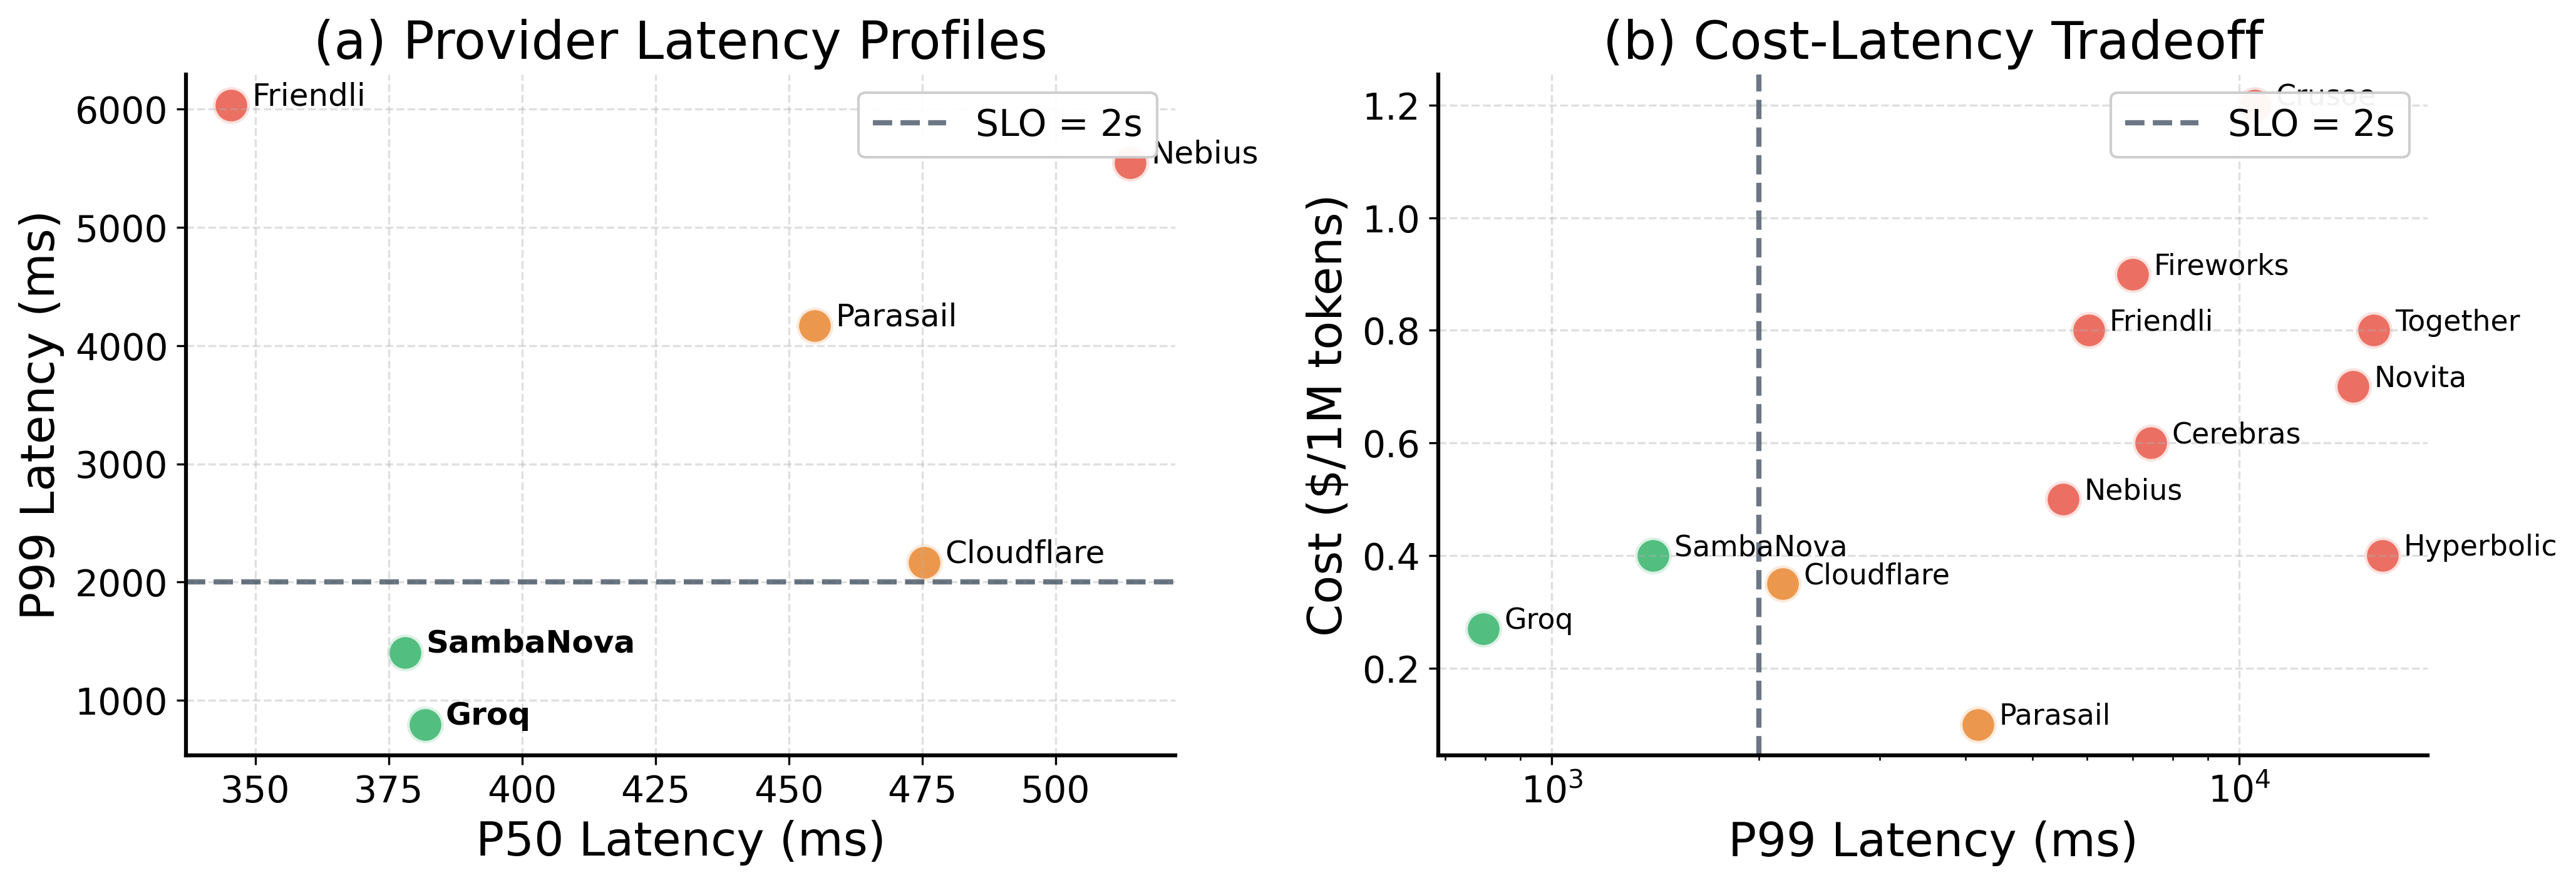
\includegraphics[width=0.9\textwidth]{images/latency_pareto_openrouter.png}
\caption{Provider latency profiles on OpenRouter (Llama-3.3-70B-Instruct). (a) P50 vs P99 latency showing provider reliability. (b) Cost-latency tradeoff---fast providers (Groq, SambaNova) meet tight SLOs but cost more; slower providers offer savings when SLOs are relaxed.}
\label{fig:latency_pareto}
\end{center}
\end{figure}

\paragraph{Online Latency Evaluation Setup.}
\label{app:latency_eval_setup}

We evaluate our latency-aware routing on the OpenRouter platform, which provides access to the same model (Llama-3.3-70B-Instruct) across 12+ providers with different latency and cost profiles.

\textbf{Model and Workload.} We use \texttt{meta-llama/llama-3.3-70b-instruct} served via OpenRouter. The workload combines BurstGPT arrival timestamps (realistic request patterns) with ShareGPT prompts (real user queries), replayed over 24 hours.

\textbf{Policies Compared.} We evaluate the following routing strategies:
\begin{itemize}
    \item \textbf{OpenRouter Auto}: OpenRouter's default routing (baseline). We do not specify a provider, allowing OpenRouter to select automatically.
    \item \textbf{Fastest Fixed}: Always route to the fastest provider (Groq) regardless of cost.
    \item \textbf{Cheapest Fixed}: Always route to the cheapest provider (Parasail) regardless of latency.
    \item \textbf{LP-Mix}: Our LP-based provider mixing (Section~\ref{sec:latency}) that constructs a cost-latency Pareto-optimal distribution over providers.
    \item \textbf{Smart Hedge}: LP-Mix as primary routing, with survival-analysis-based hedging (Eq.~\ref{eq:hedge_survival}) that triggers a backup request to the fastest provider when the primary exceeds its P90 latency threshold.
\end{itemize}

\textbf{Fairness Protocol.} To ensure fair comparison, each trace request is sent to \emph{all} policies simultaneously. This guarantees that all policies experience identical network conditions and provider load for the same request, enabling direct comparison of routing decisions.

\textbf{SLO Definition.} We define the latency SLO as Time-To-First-Token (TTFT) $\le$ 2 seconds. A request violates the SLO if TTFT exceeds 2s or the request fails.

\paragraph{Cancel-Aware Cost Analysis.}
\label{app:cancel_aware}
When hedging triggers, both the primary and backup requests are in flight. If we wait for whichever completes first, the naive cost is $c_{\text{primary}} + c_{\text{backup}}$. However, major LLM providers support request cancellation by closing the HTTP connection, which stops token generation and billing.

\textbf{Cancel-aware cost model.} When the first response arrives, we cancel the other request. Let $p_{\text{hedge}}$ be the hedge rate (fraction of requests that trigger hedging). The cancel-aware cost is:
\begin{equation}
    C_{\text{cancel}} = (1 - p_{\text{hedge}}) \cdot c_{\text{primary}} + p_{\text{hedge}} \cdot c_{\text{winner}}
\end{equation}
where $c_{\text{winner}}$ is the cost of whichever request completes first. Without cancellation:
\begin{equation}
    C_{\text{no\text{-}cancel}} = (1 - p_{\text{hedge}}) \cdot c_{\text{primary}} + p_{\text{hedge}} \cdot (c_{\text{primary}} + c_{\text{backup}})
\end{equation}

\paragraph{24-Hour Evaluation Results.}

We ran a 24-hour online evaluation with 7,299 requests per policy. Table~\ref{tab:latency_full_results} shows the complete results.

\begin{table}[h]
\centering
\caption{24-Hour Online Evaluation Results (Llama-3.3-70B-Instruct, SLO = 2s TTFT)}
\label{tab:latency_full_results}
\begin{tabular}{lccccc}
\toprule
Strategy & P50 (ms) & P99 (ms) & SLO Viol. & Cost \\
\midrule
OpenRouter Auto & 820 & 7,828 & 23.8\% & \$1.81 \\
Fastest Fixed (Groq) & 307 & 1,078 & 2.2\% & \$1.82 \\
Cheapest Fixed (Parasail) & 564 & 125,156 & 56.2\% & \$0.42 \\
LP-Mix & 418 & 3,659 & 5.3\% & \$0.98 \\
Smart Hedge (Ours) & 419 & 1,431 & 0.8\% & \$1.15$^\dagger$ \\
\bottomrule
\end{tabular}
\vspace{0.5em}
\raggedright
\small{$^\dagger$ Cancel-aware cost. Without cancellation: \$1.32. Hedge triggered on 15.6\% of requests.}
\end{table}

\textbf{Key findings:}
\begin{itemize}
    \item Smart Hedge reduces SLO violations by 31$\times$ (0.8\% vs 23.8\%) and P99 latency by 5.5$\times$ (1.4s vs 7.8s) compared to OpenRouter Auto.
    \item With cancel-aware cost accounting, Smart Hedge saves 37\% cost (\$1.15 vs \$1.81) while dramatically improving latency.
    \item LP-Mix alone (without hedging) reduces cost to \$0.98 but has higher SLO violations (5.3\%) due to occasional provider slowdowns.
    \item The hedge rate of 15.6\% indicates that hedging is triggered selectively, only when the primary provider shows signs of delay.
\end{itemize}

\textbf{Implementation note.} Not all providers support mid-stream cancellation uniformly. We recommend implementing a timeout-based fallback: if cancellation fails, the backup request runs to completion but its output is discarded.

\paragraph{Proof of Proposition~\ref{prop:lp_sparsity}.}
\label{app:lp_sparsity_proof}
We provide a short proof of the sparsity claim in Section~\ref{sec:latency}.
\begin{proof}
Consider the linear program~\eqref{eq:lp_obj}--\eqref{eq:lp_slo}. Introduce a slack variable $s \ge 0$ to rewrite the SLO constraint as an equality:
\[
\sum_{j \in \mathcal{P}} \pi_j F_j(L) - s = 1 - \alpha.
\]
Together with $\sum_{j \in \mathcal{P}} \pi_j = 1$, the problem has two equality constraints in the variables $(\pi_1, \ldots, \pi_n, s)$, plus nonnegativity constraints.

Any extreme point (basic feasible solution) therefore has at most two basic variables. If $s > 0$ (the SLO constraint is slack), then at most one $\pi_j$ can be positive, yielding a single-provider solution. Otherwise $s = 0$ and at most two $\pi_j$ can be positive. In all cases, the optimal solution can be chosen to have at most two non-zero components.
\end{proof}

\paragraph{Alternative: Residual Life Decision Rule.}
An alternative to the survival-based hedging rule~\eqref{eq:hedge_survival} is based on expected residual life. Given elapsed time $t$, we compute:
\[
\mathbb{E}[\text{Remaining} \mid T > t] = \frac{\int_t^\infty (s - t) f(s) ds}{1 - F(t)}
\]
and hedge when:
\[
t + \mathbb{E}[\text{Remaining} \mid T > t] + \delta + \mathbb{E}[T_{\text{backup}}] > L_{\text{SLO}}
\]
This rule hedges when the expected completion time exceeds the SLO. In practice, the survival-based rule~\eqref{eq:hedge_survival} performs slightly better as it directly optimizes violation probability rather than expected latency.

\paragraph{Hedging Strategy Comparison.}
Table~\ref{tab:hedging_strategies} compares different hedging strategies:
\begin{table}[h]
\caption{Hedging Strategy Comparison}
\label{tab:hedging_strategies}
\begin{center}
\begin{tabular}{lccc}
\toprule
Strategy & Cost Overhead & P99 Reduction & Description \\
\midrule
Never & 1.0$\times$ & 0\% & LP-mix only \\
Always & 2.0$\times$ & Optimal & Send two requests always \\
Fixed-$\alpha$ & 1.2--1.5$\times$ & Good & Hedge at $t = \alpha \cdot L_{\text{SLO}}$ \\
Smart (Ours) & 1.1--1.3$\times$ & Near-optimal & Hedge via~\eqref{eq:hedge_survival} \\
\bottomrule
\end{tabular}
\end{center}
\end{table}

\paragraph{Pre-filtering for Robustness.}
Before solving the LP, we filter out clearly unusable providers:
\begin{enumerate}
    \item Error rate $> 5\%$ in the recent window (clearly broken)
    \item $F_j(L_{\min}) < 80\%$ where $L_{\min} = 1$s (cannot meet basic SLO)
\end{enumerate}
This prevents the LP from routing to unreliable providers even if they are cheap.

\paragraph{LP Relaxation Fallback.}
If the LP is infeasible (no provider mix achieves the target CDF), we progressively relax the SLO:
\begin{enumerate}
    \item Try $1.2 \times L_{\text{SLO}}$
    \item Try $1.5 \times L_{\text{SLO}}$
    \item Try $2.0 \times L_{\text{SLO}}$
    \item Best-effort: select the provider with highest $F_j(L_{\text{SLO}})$
\end{enumerate}

\paragraph{Smooth Weighted Round-Robin (SWRR).}
The LP outputs routing probabilities $\pi^*$, but we need to convert these to actual routing decisions. Rather than sampling randomly (which has high short-term variance), we use SWRR:
\begin{algorithm}[H]
\caption{Smooth Weighted Round-Robin (SWRR)}
\label{alg:swrr}
\begin{algorithmic}
\STATE Initialize: $\text{cw}[j] \gets 0$ for all $j$
\FOR{each request}
    \STATE $\text{cw}[j] \gets \text{cw}[j] + \pi_j$ for all $j$
    \STATE Select $j^* = \arg\max_j \text{cw}[j]$
    \STATE $\text{cw}[j^*] \gets \text{cw}[j^*] - 1$
    \STATE Route to $j^*$
\ENDFOR
\end{algorithmic}
\end{algorithm}
SWRR produces deterministic interleaving (e.g., $\pi = [0.7, 0.3]$ yields ``AABABAA...'' rather than random bursts), reducing short-term latency variance.

% =============================================================================
\subsection{Hyperparameter Sensitivity Analysis}
\label{app:hyperparameters}

We analyze the sensitivity of our algorithms to key hyperparameters.

\paragraph{Value Bounds ($L$, $U$).}
The threshold function $\psi(z) = L \cdot (U/L)^z$ depends on the estimated value bounds. Table~\ref{tab:lu_sensitivity} shows how different choices of $L$ and $U$ affect the competitive ratio on BurstGPT.

\begin{table}[h]
\caption{Sensitivity to Value Bounds $[L, U]$ (BurstGPT)}
\label{tab:lu_sensitivity}
\begin{center}
\begin{tabular}{cccc}
\toprule
$L$ (percentile) & $U$ (percentile) & CR & API Cost \\
\midrule
1st & 99th & 1.21 & \$642 \\
5th & 95th & \textbf{1.18} & \textbf{\$629} \\
10th & 90th & 1.19 & \$635 \\
25th & 75th & 1.24 & \$661 \\
\bottomrule
\end{tabular}
\end{center}
\end{table}

\textbf{Finding:} The 5th/95th percentile bounds perform best. Tighter bounds (10th/90th, 25th/75th) reduce the effective range of the threshold, making the algorithm less adaptive. Wider bounds (1st/99th) are sensitive to outliers.

\paragraph{EMA Smoothing Factor ($\alpha$).}
The EMA predictor's responsiveness is controlled by $\alpha$. Higher $\alpha$ adapts faster but is noisier.

\begin{table}[h]
\caption{Sensitivity to EMA Smoothing Factor $\alpha$ (BurstGPT)}
\label{tab:alpha_sensitivity}
\begin{center}
\begin{tabular}{ccc}
\toprule
$\alpha$ & CR & Notes \\
\midrule
0.01 & 1.23 & Too slow to adapt \\
0.05 & 1.20 & Moderate adaptation \\
0.10 & \textbf{1.18} & Best balance \\
0.20 & 1.19 & Slightly noisy \\
0.50 & 1.25 & Too reactive \\
\bottomrule
\end{tabular}
\end{center}
\end{table}

\textbf{Finding:} $\alpha = 0.1$ provides the best balance between responsiveness and stability. This corresponds to an effective window of approximately 10 recent samples.

\paragraph{Quota Size ($Q$).}
We vary the daily quota from 1,000 to 20,000 and measure the gap between Greedy and Optimal.

\begin{table}[h]
\caption{Effect of Quota Size on Greedy vs Optimal Gap (ShareGPT)}
\label{tab:quota_sensitivity}
\begin{center}
\begin{tabular}{cccc}
\toprule
Quota $Q$ & Greedy Savings & Optimal Savings & Gap \\
\midrule
1,000 & 8\% & 12\% & 4\% \\
2,000 & 15\% & 22\% & 7\% \\
5,000 & 17\% & 35\% & 18\% \\
10,000 & 18\% & 42\% & 24\% \\
20,000 & 18\% & 48\% & 30\% \\
\bottomrule
\end{tabular}
\end{center}
\end{table}

\textbf{Finding:} The gap between Greedy and Optimal widens as quota increases. With small quotas, both strategies are capacity-constrained. With large quotas, Optimal can be highly selective while Greedy wastes capacity on low-value requests.

% =============================================================================
\subsection{Worked Routing Example}
\label{app:worked_example}

We illustrate the primal-dual routing algorithm with a concrete example.

\paragraph{Setup.}
Consider a day with quota $Q = 3$ and value bounds $[L, U] = [\$0.10, \$1.00]$. Five requests arrive sequentially:

\begin{center}
\begin{tabular}{cccc}
\toprule
Request & Input Tokens & Output Tokens & API Cost \\
\midrule
$r_1$ & 500 & 200 & \$0.15 \\
$r_2$ & 1000 & 800 & \$0.45 \\
$r_3$ & 200 & 100 & \$0.08 \\
$r_4$ & 2000 & 1500 & \$0.85 \\
$r_5$ & 800 & 600 & \$0.38 \\
\bottomrule
\end{tabular}
\end{center}

\paragraph{Greedy Routing.}
Greedy accepts requests in order until quota exhausted:
\begin{center}
\begin{tabular}{ccccc}
$r_1$ & $r_2$ & $r_3$ & $r_4$ & $r_5$ \\
$S_Q$ & $S_Q$ & $S_Q$ & API & API \\
\end{tabular}
\end{center}
Total API cost: $\$0.85 + \$0.38 = \$1.23$. Savings: $\$0.15 + \$0.45 + \$0.08 = \$0.68$.

\paragraph{Primal-Dual Routing.}
We apply the threshold function $\psi(z) = 0.10 \cdot 10^z$:

\textbf{Request $r_1$:} $z = 0/3 = 0$, $\psi(0) = \$0.10$. Value $\$0.15 > \$0.10$. \textcolor{green}{Accept} ($k=1$).

\textbf{Request $r_2$:} $z = 1/3 = 0.33$, $\psi(0.33) = \$0.22$. Value $\$0.45 > \$0.22$. \textcolor{green}{Accept} ($k=2$).

\textbf{Request $r_3$:} $z = 2/3 = 0.67$, $\psi(0.67) = \$0.46$. Value $\$0.08 < \$0.46$. \textcolor{red}{Reject} (route to API).

\textbf{Request $r_4$:} $z = 2/3 = 0.67$, $\psi(0.67) = \$0.46$. Value $\$0.85 > \$0.46$. \textcolor{green}{Accept} ($k=3$).

\textbf{Request $r_5$:} Quota exhausted. Route to API.

\begin{center}
\begin{tabular}{ccccc}
$r_1$ & $r_2$ & $r_3$ & $r_4$ & $r_5$ \\
$S_Q$ & $S_Q$ & API & $S_Q$ & API \\
\end{tabular}
\end{center}
Total API cost: $\$0.08 + \$0.38 = \$0.46$. Savings: $\$0.15 + \$0.45 + \$0.85 = \$1.45$.

\paragraph{Comparison.}
Primal-Dual saves \$1.45 vs Greedy's \$0.68 (2.1x improvement). By rejecting the low-value $r_3$ (\$0.08), it reserved quota for the high-value $r_4$ (\$0.85).

% =============================================================================
\subsection{Implementation Details}
\label{app:implementation}

\paragraph{Software Stack.}
Our implementation uses Python 3.10 with the following key libraries:
\begin{center}
\begin{tabular}{ll}
\toprule
Component & Library/Tool \\
\midrule
ILP Solver & Gurobi 10.0 (academic license) \\
Data Processing & Pandas 2.0, NumPy 1.24 \\
Visualization & Matplotlib 3.7 \\
Experiment Tracking & Custom YAML configuration \\
\bottomrule
\end{tabular}
\end{center}

\paragraph{ILP Solver Performance.}
Table~\ref{tab:ilp_runtime} shows the ILP solve time for different problem sizes.

\begin{table}[h]
\caption{ILP Solve Time vs Problem Size}
\label{tab:ilp_runtime}
\begin{center}
\begin{tabular}{ccccc}
\toprule
Requests & Time Slots & Variables & Constraints & Solve Time \\
\midrule
100 & 1,000 & 10K & 5K & 0.5s \\
500 & 5,000 & 250K & 25K & 8s \\
1,000 & 10,000 & 1M & 50K & 45s \\
5,000 & 50,000 & 25M & 250K & 12min \\
\bottomrule
\end{tabular}
\end{center}
\end{table}

\paragraph{Online Algorithm Latency.}
The online routing decision is extremely fast:
\begin{center}
\begin{tabular}{lc}
\toprule
Operation & Latency \\
\midrule
EMA prediction & $< 1\mu s$ \\
Histogram lookup & $\sim 10\mu s$ \\
Threshold computation & $< 1\mu s$ \\
Total routing decision & $< 50\mu s$ \\
\bottomrule
\end{tabular}
\end{center}

This overhead is negligible compared to typical LLM inference latency (seconds).

\paragraph{Reproducibility.}
All experiments were run on a server with Intel Xeon E5-2680 v4 (28 cores), 256GB RAM. Random seeds were fixed for reproducibility. The complete codebase and experiment configurations are available at the project repository.

% =============================================================================
\subsection{Extended Experimental Results}
\label{app:extended_results}

\paragraph{Stage 1 Cost Savings.}
Table~\ref{tab:stage1_savings} summarizes the cost savings of different strategies relative to the All-API baseline across all datasets.

\begin{table}[h]
\caption{API Cost Savings vs All-API (Quota-Only)}
\label{tab:stage1_savings}
\begin{center}
\begin{small}
\begin{sc}
\begin{tabular}{lccc}
\toprule
Dataset & Greedy & Optimal & CR \\
\midrule
ShareGPT & 17\% & \textbf{35\%} & 1.43x \\
FreeInference & 63\% & \textbf{82\%} & 1.36x \\
Enterprise & 81\% & \textbf{98\%} & 4.36x \\
\bottomrule
\end{tabular}
\end{sc}
\end{small}
\end{center}
\end{table}

\paragraph{Additional Analysis.}
Per-day results on ShareGPT show consistent performance: PD-EMA achieves CR 1.03--1.04 across all 7 days, while Greedy varies between 1.10--1.16. For multi-model workloads (FreeInference), the Greedy-Optimal gap is consistent across models (18--19\%), but absolute savings are larger for expensive models (GPT-4: \$0.76/req vs Mistral-7B: \$0.05/req). Workloads with higher output length variance (CV) show larger optimization potential: Enterprise (CV=2.4) has the largest gap, while ShareGPT (CV=1.2) has the smallest.

\paragraph{Failure Case Analysis.}
We identify scenarios where our algorithm underperforms:

\textbf{(1) Adversarial arrival order.} If high-value requests always arrive early and low-value requests arrive late, the primal-dual algorithm may over-accept early, leaving insufficient quota for (hypothetical) even higher value requests. In practice, request values are not adversarially ordered.

\textbf{(2) Highly non-stationary workloads.} When the output length distribution changes dramatically within a single quota window, both EMA and histogram predictors lag. This is rare in production workloads.

\textbf{(3) Very small quotas.} When $Q$ is very small (e.g., $Q < 100$), the threshold function has limited range, reducing the benefit of adaptive routing.


\end{document}
